\documentclass[11pt, letterpaper]{article}

% Fonts and Encoding
\usepackage[utf8]{inputenc}
\usepackage[T1]{fontenc}
\usepackage{lmodern} % High-quality Latin Modern vector font

% Math and Symbols
\usepackage{amsmath, amssymb, amsthm, amsfonts, mathrsfs, mathtools}

% Layout and Geometry
\usepackage{geometry}
\geometry{letterpaper, margin=1in}
\setlength{\parindent}{0pt}
\setlength{\parskip}{0.6em}

% Formatting and Graphics
\usepackage{graphicx, xcolor, enumitem, booktabs, array, tabularx}

% TikZ for Illustrations
\usepackage{tikz}
\usetikzlibrary{arrows.meta, positioning, shapes.geometric, calc, backgrounds, matrix}

% Clickable Links and TOC
\usepackage{hyperref}
\hypersetup{
    colorlinks=true,
    linkcolor=blue,
    filecolor=magenta,      
    urlcolor=cyan,
    pdftitle={Advanced Mathematics Topic},
}

% Theorem Environments
\newtheorem{theorem}{Theorem}[section]
\newtheorem{lemma}[theorem]{Lemma}
\newtheorem{proposition}[theorem]{Proposition}
\newtheorem{corollary}[theorem]{Corollary}
\theoremstyle{definition}
\newtheorem{definition}{Definition}[section]
\newtheorem{axiom}{Axiom}[section]
\newtheorem{example}{Example}[section]
\theoremstyle{remark}
\newtheorem{remark}{Remark}[section]

% Custom Commands (Enforced standard notation)
\newcommand{\R}{\mathbb{R}}
\newcommand{\N}{\mathbb{N}}
\newcommand{\Z}{\mathbb{Z}}
\newcommand{\Q}{\mathbb{Q}}
\newcommand{\E}{\mathbb{E}}
\newcommand{\Prob}{\mathbb{P}}
\newcommand{\F}{\mathcal{F}}

\title{\textbf{Functions of Random Variables, Sampling Distributions, and Measure-Theoretic Foundations of Statistical Inference}}
\author{Tashfeen Omran}
\date{\today}

\begin{document}

\maketitle
\tableofcontents
\newpage

% ============================================================================
% PART 1: COMPREHENSIVE INTRODUCTION, CONTEXT, AND PREREQUISITES
% ============================================================================
\section{Comprehensive Introduction, Context, and Prerequisites}

\subsection{Core Concepts and Axioms}

The primary objective of mathematical statistics is to formulate rigorous inductive inferences about an unknown population probability measure based on finite, empirical observations drawn from that population. In Sections 6.1 and 6.2 of our source text, we transition from the study of isolated random variables to the study of \emph{functions of random variables}—the mathematical objects that serve as estimators, test statistics, and decision rules.

To treat this subject with the rigor of modern abstract mathematics, we must ground every statistical concept in measure-theoretic probability.

\begin{axiom}[Probability Space]
A \emph{probability space} is a measure-theoretic triple $(\Omega, \F, \Prob)$, where:
\begin{enumerate}[label=(\roman*)]
    \item $\Omega$ is a non-empty set called the \emph{sample space}, whose elements $\omega \in \Omega$ represent elementary outcomes.
    \item $\F \subseteq \mathcal{P}(\Omega)$ is a \emph{$\sigma$-algebra} of subsets of $\Omega$ (called \emph{events}), satisfying:
    \begin{enumerate}[label=(\alph*)]
        \item $\Omega \in \F$;
        \item If $A \in \F$, then its complement $A^c = \Omega \setminus A \in \F$;
        \item If $\{A_k\}_{k=1}^{\infty} \subset \F$, then the countable union $\bigcup_{k=1}^{\infty} A_k \in \F$.
    \end{enumerate}
    \item $\Prob : \F \to [0, 1]$ is a \emph{probability measure} satisfying Kolmogorov's axioms:
    \begin{enumerate}[label=(\alph*)]
        \item Non-negativity: $\Prob(A) \ge 0$ for all $A \in \F$;
        \item Normalization: $\Prob(\Omega) = 1$;
        \item Countable Additivity ($\sigma$-additivity): If $\{A_k\}_{k=1}^{\infty} \subset \F$ are pairwise disjoint ($A_i \cap A_j = \emptyset$ for $i \neq j$), then
        \[
            \Prob\left(\bigcup_{k=1}^{\infty} A_k\right) = \sum_{k=1}^{\infty} \Prob(A_k).
        \]
    \end{enumerate}
\end{enumerate}
\end{axiom}

\begin{definition}[Random Variable and Random Vector]
Let $(\Omega, \F, \Prob)$ be a probability space, and let $(\R^n, \mathcal{B}(\R^n))$ be the $n$-dimensional Euclidean space equipped with its Borel $\sigma$-algebra $\mathcal{B}(\R^n)$ (the smallest $\sigma$-algebra containing all open subsets of $\R^n$). A mapping $\mathbf{Y} = (Y_1, Y_2, \dots, Y_n)^T : \Omega \to \R^n$ is an \emph{$n$-dimensional random vector} if it is $(\F, \mathcal{B}(\R^n))$-measurable; that is, for every Borel set $B \in \mathcal{B}(\R^n)$, its pre-image lies in $\F$:
\[
    \mathbf{Y}^{-1}(B) \coloneqq \{\omega \in \Omega : \mathbf{Y}(\omega) \in B\} \in \F.
\]
When $n = 1$, $Y : \Omega \to \R$ is called a \emph{random variable}.
\end{definition}

\begin{definition}[Pushforward Measure / Induced Probability Distribution]
Given a random vector $\mathbf{Y} : \Omega \to \R^n$, the \emph{induced probability distribution} (or \emph{pushforward measure}) $\Prob_{\mathbf{Y}} : \mathcal{B}(\R^n) \to [0, 1]$ is defined for all $B \in \mathcal{B}(\R^n)$ by
\[
    \Prob_{\mathbf{Y}}(B) \coloneqq \Prob\left(\mathbf{Y}^{-1}(B)\right) = \Prob\left(\{\omega \in \Omega : (Y_1(\omega), \dots, Y_n(\omega)) \in B\}\right).
\]
If $\Prob_{\mathbf{Y}}$ is absolutely continuous with respect to the $n$-dimensional Lebesgue measure $\lambda_n$ (denoted $\Prob_{\mathbf{Y}} \ll \lambda_n$), then by the Radon-Nikodym Theorem there exists a non-negative Borel-measurable function $f_{\mathbf{Y}} : \R^n \to [0, \infty)$, called the \emph{joint probability density function} (joint PDF), such that for all $B \in \mathcal{B}(\R^n)$,
\[
    \Prob_{\mathbf{Y}}(B) = \int_{B} f_{\mathbf{Y}}(y_1, y_2, \dots, y_n) \, d\lambda_n(y_1, \dots, y_n).
\]
If the support of $\mathbf{Y}$ is a countable set $\mathcal{S} \subset \R^n$, $\Prob_{\mathbf{Y}}$ is discrete and is characterized by the \emph{joint probability mass function} (joint PMF) $p_{\mathbf{Y}}(y_1, \dots, y_n) = \Prob(Y_1 = y_1, \dots, Y_n = y_n)$.
\end{definition}

\begin{definition}[Function of Random Variables and Statistic]
Let $\mathbf{Y} = (Y_1, \dots, Y_n)^T : \Omega \to \R^n$ be a random vector and let $g : \R^n \to \R^m$ be a Borel-measurable function, meaning $g^{-1}(A) \in \mathcal{B}(\R^n)$ for every $A \in \mathcal{B}(\R^m)$. Then the composite mapping
\[
    \mathbf{U} \coloneqq g \circ \mathbf{Y} = g(Y_1, Y_2, \dots, Y_n) : \Omega \to \R^m
\]
is an $m$-dimensional random vector. When $m=1$ and the function $g : \R^n \to \R$ does not depend on any unknown population parameters, the random variable $U = g(Y_1, \dots, Y_n)$ is called a \emph{statistic} or an \emph{estimator}. Its induced probability measure $\Prob_U = \Prob_{\mathbf{Y}} \circ g^{-1}$ is called the \emph{sampling distribution} of the statistic $U$.
\end{definition}

\begin{definition}[Independent and Identically Distributed (I.I.D.) Random Sample]
The random variables $Y_1, Y_2, \dots, Y_n$ are said to form a \emph{random sample of size $n$} from a population with marginal distribution $\Prob_Y$ (having density $f(y)$ in the continuous case or mass function $p(y)$ in the discrete case) if:
\begin{enumerate}[label=(\roman*)]
    \item \textbf{Mutual Independence:} For any collection of Borel sets $B_1, B_2, \dots, B_n \in \mathcal{B}(\R)$,
    \[
        \Prob\left(\bigcap_{i=1}^{n} \{Y_i \in B_i\}\right) = \prod_{i=1}^{n} \Prob(Y_i \in B_i),
    \]
    which implies that the joint distribution measure is the product measure $\Prob_{\mathbf{Y}} = \bigotimes_{i=1}^{n} \Prob_{Y_i}$.
    \item \textbf{Identical Distribution:} Each $Y_i$ has the identical marginal probability measure $\Prob_{Y_i} = \Prob_Y$, so that
    \[
        f(y_1, y_2, \dots, y_n) = \prod_{i=1}^{n} f(y_i) \quad \text{(continuous)} \qquad \text{or} \qquad p(y_1, y_2, \dots, y_n) = \prod_{i=1}^{n} p(y_i) \quad \text{(discrete)}.
    \]
\end{enumerate}
\end{definition}

\begin{definition}[Sample Mean and Error of Estimation]
Given a random sample $Y_1, Y_2, \dots, Y_n$ from a population with unknown mean $\mu = \E[Y_i]$, the \emph{sample mean} is the linear functional statistic
\[
    \bar{Y} = g(Y_1, Y_2, \dots, Y_n) \coloneqq \frac{1}{n} \sum_{i=1}^{n} Y_i.
\]
For a specific realization $(y_1, y_2, \dots, y_n) \in \R^n$, the realized numerical value $\bar{y} = \frac{1}{n}\sum_{i=1}^n y_i$ is called an \emph{estimate} of $\mu$, whereas the random variable $\bar{Y}$ is the \emph{estimator}. The \emph{error of estimation} is the random variable
\[
    \mathcal{E} \coloneqq |\bar{Y} - \mu|.
\]
The statistical goodness of $\bar{Y}$ is quantified by the tail probability $\Prob(|\bar{Y} - \mu| \le B)$ for a specified tolerance bound $B > 0$.
\end{definition}

\subsection{Intuition and Set-Theoretic/Logical Foundations}

Why must we obsess over the probability distribution of a function $U = g(Y_1, \dots, Y_n)$ rather than simply computing a single numerical average $\bar{y}$ from data? 

From a set-theoretic perspective, an experiment selects a single elementary outcome $\omega \in \Omega$ according to the measure $\Prob$. The random sample $\mathbf{Y} = (Y_1, \dots, Y_n)$ projects this abstract outcome $\omega$ into a point $\mathbf{y} = (y_1, \dots, y_n)$ in the $n$-dimensional Euclidean observation space $\R^n$. However, an $n$-dimensional cloud of numbers is difficult to interpret directly when estimating a scalar parameter $\mu \in \R$. Thus, we apply a data-reduction mapping $g : \R^n \to \R$ (such as the sample mean $g(\mathbf{y}) = \frac{1}{n}\sum_{i=1}^n y_i$), which collapses hyperplanes of $\R^n$ onto single points $u \in \R$.

To find the probability that our compressed summary $U$ falls into an interval $A = [\mu - B, \mu + B] \subset \R$, we must trace the set $A$ backward through the function $g$ into $\R^n$. The pre-image
\[
    g^{-1}(A) = \left\{(y_1, \dots, y_n) \in \R^n : \mu - B \le \frac{1}{n}\sum_{i=1}^{n} y_i \le \mu + B\right\}
\]
is a geometric slab bounded by two parallel $(n-1)$-dimensional hyperplanes in $\R^n$. Finding the distribution of $U$ is equivalent to integrating the joint density $f(y_1, \dots, y_n) = \prod_{i=1}^n f(y_i)$ over these geometric level sets in $\R^n$. Each of the four methods introduced in Section 6.2 (Distribution Functions, Transformations, Moment-Generating Functions, and Jacobians) is a specialized analytical machinery designed to evaluate or bypass this $n$-dimensional pre-image integral cleanly.

\subsection{Historical Context and Motivation}

The formal study of functions of random variables emerged from the crisis of observational error in eighteenth- and nineteenth-century astronomy and geodesy. Pioneers such as Thomas Simpson (1755), Pierre-Simon Laplace (1774--1812), and Carl Friedrich Gauss (1809) sought to justify why the arithmetic mean $\bar{y} = \frac{1}{n}\sum_{i=1}^n y_i$ of repeated astronomical measurements provided a superior estimate of a celestial body's true position compared to a single observation. Laplace developed the method of characteristic functions (the complex-analytic precursor to moment-generating functions) specifically to derive the probability distribution of linear combinations of independent errors, culminating in the earliest versions of the Central Limit Theorem.

In the early twentieth century, William Sealy Gosset (writing under the pseudonym ``Student'' in 1908) and Sir Ronald A. Fisher (1915--1925) realized that asymptotic approximations were inadequate for small sample sizes $n$ encountered in agricultural and industrial experiments. By employing geometric $n$-dimensional transformations and Jacobian determinants, Gosset and Fisher derived the exact finite-sample distributions of non-linear functions of Gaussian random variables—yielding the celebrated Student's $t$, Chi-square ($\chi^2$), and Fisher-Snedecor $F$ distributions. Finally, in 1933, Andrey Kolmogorov published \emph{Grundbegriffe der Wahrscheinlichkeitsrechnung}, unifying these geometric and analytical techniques under Lebesgue's theory of measure and integration, thereby establishing that random variables are measurable functions and sampling distributions are pushforward measures.

\subsection{Key Theorems, Lemmas, and Formulas}

\begin{theorem}[Measurability of Composite Functions]
\label{thm:composite_measurability}
Let $(\Omega, \F, \Prob)$ be a probability space, let $\mathbf{Y} : \Omega \to \R^n$ be an $(\F, \mathcal{B}(\R^n))$-measurable random vector, and let $g : \R^n \to \R^m$ be a $(\mathcal{B}(\R^n), \mathcal{B}(\R^m))$-measurable mapping. Then $\mathbf{U} = g \circ \mathbf{Y} : \Omega \to \R^m$ is an $(\F, \mathcal{B}(\R^m))$-measurable random vector. In particular, every continuous function $g : \R^n \to \R^m$ is Borel-measurable.
\end{theorem}

\begin{theorem}[The Four Fundamental Methods for Deriving Sampling Distributions]
Let $\mathbf{Y} = (Y_1, \dots, Y_n)^T$ have joint density $f_{\mathbf{Y}}(y_1, \dots, y_n)$ and let $U = g(Y_1, \dots, Y_n)$.
\begin{enumerate}[label=\textbf{\arabic*.}]
    \item \textbf{Method of Distribution Functions (CDF Method):} For any $u \in \R$, the cumulative distribution function of $U$ is obtained by integrating the joint density over the pre-image region $R_u = \{\mathbf{y} \in \R^n : g(\mathbf{y}) \le u\}$:
    \[
        F_U(u) \coloneqq \Prob(U \le u) = \idotsint\limits_{\{g(y_1, \dots, y_n) \le u\}} f_{\mathbf{Y}}(y_1, \dots, y_n) \, dy_1 \cdots dy_n, \qquad f_U(u) = \frac{d}{du} F_U(u).
    \]
    \item \textbf{Method of Univariate Transformations:} If $Y$ is a scalar continuous random variable with density $f_Y(y)$ and $U = h(Y)$ is strictly monotonic and differentiable on the support of $Y$ with inverse $y = h^{-1}(u)$, then
    \[
        f_U(u) = f_Y\left(h^{-1}(u)\right) \left|\frac{d}{du} h^{-1}(u)\right|.
    \]
    \item \textbf{Method of Moment-Generating Functions (MGF Uniqueness Theorem):} Let the moment-generating function of a random variable $W$ be $M_W(t) \coloneqq \E[e^{tW}]$. If $M_U(t)$ exists on an open neighborhood $(-t_0, t_0)$ containing $0$ ($t_0 > 0$) and equals the MGF $M_V(t)$ of a known distribution for all $t \in (-t_0, t_0)$, then $\Prob_U = \Prob_V$. Moreover, if $Y_1, \dots, Y_n$ are independent and $U = \sum_{i=1}^n a_i Y_i$, then
    \[
        M_U(t) = \E\left[\exp\left(t \sum_{i=1}^{n} a_i Y_i\right)\right] = \prod_{i=1}^{n} M_{Y_i}(a_i t).
    \]
    \item \textbf{Method of Multivariable Jacobians:} Let $\mathbf{h} : \mathcal{S} \subset \R^n \to \mathcal{T} \subset \R^n$ be a $C^1$-diffeomorphism mapping the open support $\mathcal{S}$ of $\mathbf{Y}$ bijectively onto $\mathcal{T}$, with inverse $\mathbf{y} = \mathbf{h}^{-1}(\mathbf{u})$. Then the joint density of $\mathbf{U} = \mathbf{h}(\mathbf{Y})$ is
    \[
        f_{\mathbf{U}}(u_1, \dots, u_n) = f_{\mathbf{Y}}\left(h_1^{-1}(\mathbf{u}), \dots, h_n^{-1}(\mathbf{u})\right) \left|\det J_{\mathbf{h}^{-1}}(\mathbf{u})\right| \mathbf{1}_{\mathcal{T}}(\mathbf{u}),
    \]
    where $\det J_{\mathbf{h}^{-1}}(\mathbf{u}) = \frac{\partial(y_1, \dots, y_n)}{\partial(u_1, \dots, u_n)}$ is the Jacobian determinant of the inverse transformation.
\end{enumerate}
\end{theorem}

\subsection{Prerequisites}

To master this chapter at an advanced theoretical level, the reader requires proficiency in:
\begin{itemize}
    \item \textbf{Foundational Set Theory and Measure Theory:} Pre-images of functions ($f^{-1}(A \cup B) = f^{-1}(A) \cup f^{-1}(B)$, $f^{-1}(A^c) = (f^{-1}(A))^c$), $\sigma$-algebras, Borel sets, and the Fubini-Tonelli Theorem for iterated integrals over product spaces.
    \item \textbf{Multivariable Real Analysis:} Change of variables in multiple integrals, open and closed domains in $\R^n$, partial differentiation, and Leibniz's Rule for differentiating integrals with variable limits.
    \item \textbf{Linear Algebra:} Matrix determinants, invertibility of linear transformations, and Jacobian matrices.
    \item \textbf{Core Probability Theory:} Conditional probability, mutual independence, expectation operators, variance, covariance, and classical parametric families (Normal, Gamma, Exponential, Binomial, Hypergeometric).
\end{itemize}

\newpage

% ============================================================================
% PART 2: DETAILED HOMEWORK SOLUTIONS (RIGOROUS PROOFS & COMPUTATIONS)
% ============================================================================
\section{Detailed Homework Solutions: Rigorous Proofs and Computations}

\subsection{Original Source Text and Extracted Theoretical Problems}

Below is the verbatim transcription of the source material provided in the assignment (Chapter 6: \emph{Functions of Random Variables}, Sections 6.1 and 6.2, pages 296--297), followed by the five rigorous mathematical problems and proofs directly embedded in the text's theoretical claims.

\begin{quote}
\textbf{CHAPTER 6: Functions of Random Variables} \\ \relax
\textbf{6.1 Introduction} \\ \relax
As we indicated in Chapter 1, the objective of statistics is to make inferences about a population based on information contained in a sample taken from that population. Any truly useful inference must be accompanied by an associated measure of goodness. Each of the topics discussed in the preceding chapters plays a role in the development of statistical inference. However, none of the topics discussed thus far pertains to the objective of statistics as closely as the study of the distributions of functions of random variables. This is because all quantities used to estimate population parameters or to make decisions about a population are functions of the $n$ random observations that appear in a sample.

To illustrate, consider the problem of estimating a population mean, $\mu$. Intuitively we draw a random sample of $n$ observations, $y_1, y_2, \dots, y_n$, from the population and employ the sample mean
\[
    \bar{y} = \frac{y_1 + y_2 + \cdots + y_n}{n} = \frac{1}{n} \sum_{i=1}^{n} y_i
\]
as an estimate for $\mu$. How good is this estimate? The answer depends upon the behavior of the random variables $Y_1, Y_2, \dots, Y_n$ and their effect on the distribution of $\bar{Y} = (1/n) \sum_{i=1}^{n} Y_i$.

A measure of the goodness of an estimate is the \emph{error of estimation}, the difference between the estimate and the parameter estimated (for our example, the difference between $\bar{y}$ and $\mu$). Because $Y_1, Y_2, \dots, Y_n$ are random variables, in repeated sampling $\bar{Y}$ is also a random variable (and a function of the $n$ variables $Y_1, Y_2, \dots, Y_n$). Therefore, we cannot be certain that the error of estimation will be less than a specific value, say, $B$. However, if we can determine the probability distribution of the estimator $\bar{Y}$, this probability distribution can be used to determine the \emph{probability} that the error of estimation is less than or equal to $B$.

To determine the probability distribution for a function of $n$ random variables, $Y_1, Y_2, \dots, Y_n$, we must find the joint probability distribution for the random variables themselves. We generally assume that observations are obtained through random sampling, as defined in Section 2.12. We saw in Section 3.7 that random sampling from a finite population (sampling without replacement) results in dependent trials, but that these trials become essentially independent if the population is large when compared to the size of the sample.

We will assume throughout the remainder of this text that populations are large in comparison to the sample size and consequently that the random variables obtained through a random sample are in fact independent of one another. Thus, in the discrete case, the joint probability function for $Y_1, Y_2, \dots, Y_n$, all sampled from the same population, is given by
\[
    p(y_1, y_2, \dots, y_n) = p(y_1)p(y_2)\cdots p(y_n).
\]
In the continuous case, the joint density function is
\[
    f(y_1, y_2, \dots, y_n) = f(y_1)f(y_2)\cdots f(y_n).
\]
The statement ``$Y_1, Y_2, \dots, Y_n$ is a random sample from a population with density $f(y)$'' will mean that the random variables are independent with common density function $f(y)$.

\textbf{6.2 Finding the Probability Distribution of a Function of Random Variables} \\ \relax
We will present three methods for finding the probability distribution for a function of random variables and a fourth method for finding the joint distribution of several functions of random variables. Any one of these may be employed to find the distribution of a given function of the variables, but one of the methods usually leads to a simpler derivation than the others. The method that works ``best'' varies from one application to another. Hence, acquaintance with the first three methods is desirable. The fourth method is presented in (optional) Section 6.6. Although the first three methods will be discussed separately in the next three sections, a brief summary of each of these methods is provided here.
\end{quote}

---

\subsection{Problem 1: Measure-Theoretic Validity of the Sample Mean as a Random Variable}

\textbf{Original Problem Statement (Extracted from Section 6.1, Paragraph 3):} \\ \relax
The text asserts: \emph{``Because $Y_1, Y_2, \dots, Y_n$ are random variables, in repeated sampling $\bar{Y} = \frac{1}{n}\sum_{i=1}^n Y_i$ is also a random variable (and a function of the $n$ variables $Y_1, Y_2, \dots, Y_n$).''}
\begin{enumerate}[label=(\alph*)]
    \item Prove that if $\mathbf{Y} = (Y_1, \dots, Y_n)^T : \Omega \to \R^n$ is a random vector on $(\Omega, \F, \Prob)$ and $g : \R^n \to \R$ is a continuous function, then $U = g(Y_1, \dots, Y_n)$ is a valid $(\F, \mathcal{B}(\R))$-measurable random variable.
    \item Using mathematical induction and first principles of pre-images on rational cuts, prove directly that the sample mean $\bar{Y} = \frac{1}{n}\sum_{i=1}^n Y_i$ is an $\F$-measurable random variable whenever $Y_1, \dots, Y_n$ are individual random variables on $(\Omega, \F, \Prob)$.
\end{enumerate}

\subsubsection*{Solution and Proof}

\textbf{Proof Technique:} Set-Theoretic Direct Proof via Pre-Image Algebra and Mathematical Induction.

\textbf{Part (a): Measurability of Continuous Functions of Random Vectors.}
\begin{proof}
Let $(\Omega, \F, \Prob)$ be a probability space, and assume $\mathbf{Y} : \Omega \to \R^n$ is an $(\F, \mathcal{B}(\R^n))$-measurable mapping. Let $g : \R^n \to \R$ be continuous with respect to the standard Euclidean topologies on $\R^n$ and $\R$. We must prove that the composite function $U = g \circ \mathbf{Y} : \Omega \to \R$ satisfies $U^{-1}(B) \in \F$ for all $B \in \mathcal{B}(\R)$.

\textbf{Step 1: Establish that $g$ is Borel-measurable.} \\ \relax
Define the collection of subsets of $\R$ whose pre-images under $g$ are Borel sets in $\R^n$:
\[
    \mathcal{C} \coloneqq \left\{ E \subseteq \R : g^{-1}(E) \in \mathcal{B}(\R^n) \right\}.
\]
We first show that $\mathcal{C}$ is a $\sigma$-algebra on $\R$:
\begin{enumerate}[label=(\roman*)]
    \item Since $g^{-1}(\R) = \R^n$ and $\R^n \in \mathcal{B}(\R^n)$, we have $\R \in \mathcal{C}$.
    \item Suppose $E \in \mathcal{C}$, so $g^{-1}(E) \in \mathcal{B}(\R^n)$. By elementary set theory, the pre-image operator commutes with complementation:
    \[
        g^{-1}(E^c) = g^{-1}(\R \setminus E) = \R^n \setminus g^{-1}(E) = \left(g^{-1}(E)\right)^c.
    \]
    Because $\mathcal{B}(\R^n)$ is a $\sigma$-algebra and is closed under complements, $\left(g^{-1}(E)\right)^c \in \mathcal{B}(\R^n)$, which implies $E^c \in \mathcal{C}$.
    \item Suppose $\{E_k\}_{k=1}^{\infty} \subset \mathcal{C}$, so $g^{-1}(E_k) \in \mathcal{B}(\R^n)$ for every $k \in \N$. Because the pre-image operator distributes over arbitrary unions,
    \[
        g^{-1}\left(\bigcup_{k=1}^{\infty} E_k\right) = \bigcup_{k=1}^{\infty} g^{-1}(E_k).
    \]
    Since $\mathcal{B}(\R^n)$ is closed under countable unions, $\bigcup_{k=1}^{\infty} g^{-1}(E_k) \in \mathcal{B}(\R^n)$, and hence $\bigcup_{k=1}^{\infty} E_k \in \mathcal{C}$.
\end{enumerate}
Thus, $\mathcal{C}$ is a $\sigma$-algebra on $\R$. Next, let $\mathcal{O}(\R)$ denote the collection of all open subsets of $\R$. By the topological definition of continuity, for every open set $V \in \mathcal{O}(\R)$, its pre-image $g^{-1}(V)$ is an open subset of $\R^n$. Since $\mathcal{B}(\R^n)$ is generated by the open subsets of $\R^n$, every open subset of $\R^n$ belongs to $\mathcal{B}(\R^n)$. Therefore, $g^{-1}(V) \in \mathcal{B}(\R^n)$ for all $V \in \mathcal{O}(\R)$, which means $\mathcal{O}(\R) \subseteq \mathcal{C}$.

By definition, the Borel $\sigma$-algebra $\mathcal{B}(\R) = \sigma(\mathcal{O}(\R))$ is the smallest $\sigma$-algebra containing $\mathcal{O}(\R)$. Since $\mathcal{C}$ is a $\sigma$-algebra containing $\mathcal{O}(\R)$, it follows that $\mathcal{B}(\R) \subseteq \mathcal{C}$. Hence, for every $B \in \mathcal{B}(\R)$, $g^{-1}(B) \in \mathcal{B}(\R^n)$.

\textbf{Step 2: Compose the pre-images.} \\ \relax
Let $B \in \mathcal{B}(\R)$ be arbitrary. By the associativity of function composition and pre-images,
\[
    U^{-1}(B) = (g \circ \mathbf{Y})^{-1}(B) = \mathbf{Y}^{-1}\left(g^{-1}(B)\right).
\]
From Step 1, the set $A \coloneqq g^{-1}(B)$ is an element of $\mathcal{B}(\R^n)$. Since $\mathbf{Y}$ is $(\F, \mathcal{B}(\R^n))$-measurable by hypothesis, $\mathbf{Y}^{-1}(A) \in \F$. Consequently, $U^{-1}(B) \in \F$ for all $B \in \mathcal{B}(\R)$, proving that $U$ is a valid random variable.
\end{proof}

\textbf{Part (b): Direct Inductive Proof that $\bar{Y} = \frac{1}{n}\sum_{i=1}^n Y_i$ is Measurable.}
\begin{proof}
Recall the standard measure-theoretic criterion: a function $X : \Omega \to \R$ is $(\F, \mathcal{B}(\R))$-measurable if and only if for every real number $c \in \R$, the sub-level set $\{\omega \in \Omega : X(\omega) < c\} \in \F$ (since the rays $(-\infty, c)$ generate $\mathcal{B}(\R)$).

\textbf{Step 1: Prove that the sum of two random variables $S_2 = Y_1 + Y_2$ is measurable.} \\ \relax
Fix an arbitrary $c \in \R$. Consider the event
\[
    \{\omega \in \Omega : Y_1(\omega) + Y_2(\omega) < c\} = \{\omega \in \Omega : Y_1(\omega) < c - Y_2(\omega)\}.
\]
By the density of the rational numbers $\Q$ in $\R$ (the Archimedean property), for any real numbers $a, b \in \R$, we have $a < b$ if and only if there exists at least one rational number $q \in \Q$ such that $a < q < b$. Applying this equivalence pointwise for each $\omega \in \Omega$ with $a = Y_1(\omega)$ and $b = c - Y_2(\omega)$, we obtain
\begin{align*}
    \{\omega \in \Omega : Y_1(\omega) + Y_2(\omega) < c\} 
    &= \bigcup_{q \in \Q} \left( \{\omega \in \Omega : Y_1(\omega) < q\} \cap \{\omega \in \Omega : q < c - Y_2(\omega)\} \right) \\ \relax
    &= \bigcup_{q \in \Q} \left( \{\omega \in \Omega : Y_1(\omega) < q\} \cap \{\omega \in \Omega : Y_2(\omega) < c - q\} \right).
\end{align*}
Since $Y_1$ and $Y_2$ are random variables, for each fixed $q \in \Q$, the sets $E_q \coloneqq \{\omega : Y_1(\omega) < q\} \in \F$ and $F_q \coloneqq \{\omega : Y_2(\omega) < c - q\} \in \F$. Since a $\sigma$-algebra is closed under finite intersections, $E_q \cap F_q \in \F$. Furthermore, because the set of rational numbers $\Q$ is countable, $\bigcup_{q \in \Q} (E_q \cap F_q)$ is a countable union of elements of $\F$, which must belong to $\F$. Thus $S_2 = Y_1 + Y_2$ is a random variable.

\textbf{Step 2: Induction on $n$ for $S_n = \sum_{i=1}^n Y_i$.} \\ \relax
\emph{Base Case ($n=1$):} $S_1 = Y_1$ is a random variable by hypothesis. \\ \relax
\emph{Inductive Hypothesis:} Suppose for some integer $k \ge 1$ that $S_k = \sum_{i=1}^k Y_i$ is an $\F$-measurable random variable. \\ \relax
\emph{Inductive Step:} For $n = k+1$, we write $S_{k+1} = S_k + Y_{k+1}$. Since $S_k$ is a random variable by the inductive hypothesis and $Y_{k+1}$ is a random variable by hypothesis, Step 1 guarantees that their sum $S_{k+1}$ is an $\F$-measurable random variable. By the Principle of Mathematical Induction, $S_n = \sum_{i=1}^n Y_i$ is a random variable for all $n \in \N$.

\textbf{Step 3: Scalar multiplication by $1/n > 0$.} \\ \relax
For any $c \in \R$ and $n \in \N$ ($n \ge 1$),
\[
    \{\omega \in \Omega : \bar{Y}(\omega) < c\} = \left\{\omega \in \Omega : \frac{1}{n} S_n(\omega) < c\right\} = \{\omega \in \Omega : S_n(\omega) < nc\}.
\]
Since $nc \in \R$ and $S_n$ is measurable, $\{\omega \in \Omega : S_n(\omega) < nc\} \in \F$. Therefore, the sample mean $\bar{Y} = \frac{1}{n}\sum_{i=1}^n Y_i$ is a valid random variable on $(\Omega, \F, \Prob)$.
\end{proof}

---

\subsection{Problem 2: Factorization of the Joint Distribution of an I.I.D. Random Sample}

\textbf{Original Problem Statement (Extracted from Section 6.1, Paragraph 5):} \\ \relax
The text states: \emph{``Thus, in the discrete case, the joint probability function for $Y_1, Y_2, \dots, Y_n$, all sampled from the same population, is given by $p(y_1, y_2, \dots, y_n) = p(y_1)p(y_2)\cdots p(y_n)$. In the continuous case, the joint density function is $f(y_1, y_2, \dots, y_n) = f(y_1)f(y_2)\cdots f(y_n)$.''}

Prove rigorously from the measure-theoretic definition of mutual independence:
\[
    \Prob\left(\bigcap_{i=1}^{n} \{Y_i \in B_i\}\right) = \prod_{i=1}^{n} \Prob(Y_i \in B_i) \quad \forall B_1, \dots, B_n \in \mathcal{B}(\R)
\]
that if $Y_1, \dots, Y_n$ are mutually independent and identically distributed:
\begin{enumerate}[label=(\alph*)]
    \item In the discrete case with common marginal PMF $p(y) = \Prob(Y_i = y)$, the joint PMF factors as $p(y_1, \dots, y_n) = \prod_{i=1}^n p(y_i)$.
    \item In the absolutely continuous case with common marginal PDF $f(y)$, the product function $g(y_1, \dots, y_n) = \prod_{i=1}^n f(y_i)$ is the unique (up to sets of Lebesgue measure zero) joint PDF $f(y_1, \dots, y_n)$ of $(Y_1, \dots, Y_n)$.
\end{enumerate}

\subsubsection*{Solution and Proof}

\textbf{Proof Technique:} Direct Measure-Theoretic Proof utilizing Singleton Borel Sets, Fubini-Tonelli Theorem, and Dynkin's $\pi$-$\lambda$ Uniqueness Argument.

\begin{proof}
\textbf{Part (a): Discrete Factorization.} \\ \relax
Let $(y_1, y_2, \dots, y_n) \in \R^n$ be any vector in the discrete support. In the Euclidean topology on $\R$, every singleton set $\{y_i\}$ is a closed set and therefore a valid Borel set: $B_i \coloneqq \{y_i\} \in \mathcal{B}(\R)$ for each $i \in \{1, \dots, n\}$. By definition of the joint probability mass function and the axiom of mutual independence,
\begin{align*}
    p(y_1, y_2, \dots, y_n) &\coloneqq \Prob(Y_1 = y_1, Y_2 = y_2, \dots, Y_n = y_n) \\ \relax
    &= \Prob\left(\bigcap_{i=1}^{n} \{Y_i \in \{y_i\}\}\right) \\ \relax
    &= \prod_{i=1}^{n} \Prob(Y_i \in \{y_i\}) \quad \text{(by mutual independence)} \\ \relax
    &= \prod_{i=1}^{n} p_{Y_i}(y_i).
\end{align*}
Since $Y_1, \dots, Y_n$ are identically distributed with common marginal PMF $p_{Y_i}(y) = p(y)$, we substitute $p_{Y_i}(y_i) = p(y_i)$ to conclude:
\[
    p(y_1, y_2, \dots, y_n) = \prod_{i=1}^{n} p(y_i) = p(y_1)p(y_2)\cdots p(y_n).
\]

\textbf{Part (b): Continuous Density Factorization.} \\ \relax
Suppose each $Y_i$ is absolutely continuous with common marginal PDF $f(y) \ge 0$, meaning that for every Borel set $B_i \in \mathcal{B}(\R)$,
\[
    \Prob(Y_i \in B_i) = \int_{B_i} f(y_i) \, dy_i.
\]
Consider any measurable rectangle $R = B_1 \times B_2 \times \cdots \times B_n \in \mathcal{B}(\R^n)$, where $B_i \in \mathcal{B}(\R)$ for $i = 1, \dots, n$. Notice that the event $\{\mathbf{Y} \in R\}$ is precisely the intersection $\bigcap_{i=1}^n \{Y_i \in B_i\}$. Applying mutual independence and substituting the marginal density integrals yields:
\[
    \Prob_{\mathbf{Y}}(R) = \Prob\left(\bigcap_{i=1}^{n} \{Y_i \in B_i\}\right) = \prod_{i=1}^{n} \Prob(Y_i \in B_i) = \prod_{i=1}^{n} \left( \int_{B_i} f(y_i) \, dy_i \right).
\]
Since $f(y_i) \ge 0$ is Borel-measurable and non-negative on $\R$ for each $i = 1, \dots, n$, we invoke Tonelli's Theorem on the product space $(\R^n, \mathcal{B}(\R^n), \lambda_n)$ to convert the product of $n$ one-dimensional Lebesgue integrals into a single $n$-dimensional integral over $R = B_1 \times \cdots \times B_n$:
\[
    \prod_{i=1}^{n} \left( \int_{B_i} f(y_i) \, dy_i \right) = \int_{B_1} \int_{B_2} \cdots \int_{B_n} \left(\prod_{i=1}^{n} f(y_i)\right) dy_n \cdots dy_2 \, dy_1 = \int_{R} \left(\prod_{i=1}^{n} f(y_i)\right) d\lambda_n(\mathbf{y}).
\]
Thus, the probability measure $\Prob_{\mathbf{Y}}(A)$ and the set function $\nu(A) \coloneqq \int_{A} \left(\prod_{i=1}^n f(y_i)\right) d\lambda_n(\mathbf{y})$ agree on the collection $\mathcal{R} = \{B_1 \times \cdots \times B_n : B_i \in \mathcal{B}(\R)\}$ of all measurable rectangles.

Because $\mathcal{R}$ is a $\pi$-system (closed under finite intersections, since $(B_1 \times \cdots \times B_n) \cap (C_1 \times \cdots \times C_n) = (B_1 \cap C_1) \times \cdots \times (B_n \cap C_n)$) that generates the Borel $\sigma$-algebra $\mathcal{B}(\R^n) = \sigma(\mathcal{R})$, and both $\Prob_{\mathbf{Y}}$ and $\nu$ are probability measures on $\mathcal{B}(\R^n)$, Dynkin's $\pi$-$\lambda$ Theorem (or Carath\'eodory's Extension Uniqueness Theorem) guarantees that $\Prob_{\mathbf{Y}}(A) = \nu(A)$ for \emph{every} Borel set $A \in \mathcal{B}(\R^n)$:
\[
    \Prob_{\mathbf{Y}}(A) = \int_{A} \left(\prod_{i=1}^{n} f(y_i)\right) d\lambda_n(\mathbf{y}) \quad \forall A \in \mathcal{B}(\R^n).
\]
By the uniqueness of the Radon-Nikodym derivative $f_{\mathbf{Y}} = \frac{d\Prob_{\mathbf{Y}}}{d\lambda_n}$, the joint probability density function of $(Y_1, \dots, Y_n)$ is given $\lambda_n$-almost everywhere by
\[
    f(y_1, y_2, \dots, y_n) = \prod_{i=1}^{n} f(y_i) = f(y_1)f(y_2)\cdots f(y_n).
\]
\end{proof}

---

\subsection{Problem 3: Asymptotic Convergence of Finite-Population Sampling Without Replacement to I.I.D. Sampling}

\textbf{Original Problem Statement (Extracted from Section 6.1, Paragraph 4):} \\ \relax
The text states: \emph{``We saw in Section 3.7 that random sampling from a finite population (sampling without replacement) results in dependent trials, but that these trials become essentially independent if the population is large when compared to the size of the sample.''}

Let a finite dichotomous population of total size $N$ contain $M_N$ items of Type 1 (``successes'', encoded as $1$) and $N - M_N$ items of Type 0 (``failures'', encoded as $0$), such that the population proportion of successes converges to a constant $p \in (0, 1)$ as $N \to \infty$:
\[
    \lim_{N \to \infty} \frac{M_N}{N} = p.
\]
Suppose we draw an ordered random sample $(Y_1, Y_2, \dots, Y_n)$ of fixed size $n$ \emph{without replacement} from this population, where $Y_i \in \{0, 1\}$ denotes the type of the $i$-th item drawn.
\begin{enumerate}[label=(\alph*)]
    \item Prove that for any finite $N \ge n$, the random variables $Y_1$ and $Y_2$ are statistically dependent by computing $\text{Cov}(Y_1, Y_2)$.
    \item Derive the exact joint probability mass function $p_N(y_1, y_2, \dots, y_n) = \Prob_N(Y_1 = y_1, \dots, Y_n = y_n)$ for any realization $(y_1, \dots, y_n) \in \{0, 1\}^n$ with $k = \sum_{i=1}^n y_i$ successes.
    \item Prove that in the large-population limit ($N \to \infty$ with $n$ fixed), $p_N(y_1, \dots, y_n)$ converges pointwise to the joint PMF of $n$ mutually independent and identically distributed $\text{Bernoulli}(p)$ random variables:
    \[
        \lim_{N \to \infty} p_N(y_1, y_2, \dots, y_n) = \prod_{i=1}^{n} p^{y_i}(1 - p)^{1 - y_i}.
    \]
\end{enumerate}

\subsubsection*{Solution and Proof}

\textbf{Proof Technique:} Combinatorial Sequential Conditioning, Covariance Calculation, and Asymptotic Limit Analysis.

\begin{proof}
\textbf{Part (a): Proof of Dependence for Finite $N$ via Covariance.} \\ \relax
By symmetry of exchangeability in sampling without replacement, every draw $Y_i$ has the same marginal distribution as the first draw $Y_1$:
\[
    \Prob_N(Y_i = 1) = \frac{M_N}{N} \eqqcolon p_N, \qquad \E[Y_i] = p_N, \qquad \text{Var}(Y_i) = p_N(1 - p_N).
\]
For the first two draws $Y_1$ and $Y_2$, the product $Y_1 Y_2$ is non-zero (and equal to $1$) if and only if $Y_1 = 1$ and $Y_2 = 1$. By the Multiplication Rule of Conditional Probability,
\[
    \E[Y_1 Y_2] = \Prob_N(Y_1 = 1 \cap Y_2 = 1) = \Prob_N(Y_1 = 1) \Prob_N(Y_2 = 1 \mid Y_1 = 1) = \frac{M_N}{N} \cdot \frac{M_N - 1}{N - 1}.
\]
Therefore, the covariance between $Y_1$ and $Y_2$ is
\begin{align*}
    \text{Cov}(Y_1, Y_2) &= \E[Y_1 Y_2] - \E[Y_1]\E[Y_2] \\ \relax
    &= \frac{M_N(M_N - 1)}{N(N - 1)} - \left(\frac{M_N}{N}\right)^2 \\ \relax
    &= \frac{M_N\left[ N(M_N - 1) - M_N(N - 1) \right]}{N^2(N - 1)} \\ \relax
    &= \frac{M_N(M_N - N)}{N^2(N - 1)} = -\frac{p_N(1 - p_N)}{N - 1}.
\end{align*}
Since $0 < p_N < 1$ and $N < \infty$, we have $\text{Cov}(Y_1, Y_2) = -\frac{p_N(1-p_N)}{N-1} < 0 \neq 0$. Because independent random variables must have zero covariance, $Y_1$ and $Y_2$ are strictly dependent for any finite population size $N$. (Note, however, that $\lim_{N \to \infty} \text{Cov}(Y_1, Y_2) = 0$.)

\textbf{Part (b): Exact Joint PMF for Ordered Sampling Without Replacement.} \\ \relax
Let $(y_1, y_2, \dots, y_n) \in \{0, 1\}^n$ be any fixed binary sequence containing $k = \sum_{i=1}^n y_i$ ones (successes) and $n - k = \sum_{i=1}^n (1 - y_i)$ zeros (failures), where $0 \le k \le M_N$ and $0 \le n - k \le N - M_N$.

By the sequential multiplication rule:
\[
    p_N(y_1, \dots, y_n) = \Prob_N(Y_1 = y_1) \Prob_N(Y_2 = y_2 \mid Y_1 = y_1) \cdots \Prob_N(Y_n = y_n \mid Y_1 = y_1, \dots, Y_{n-1} = y_{n-1}).
\]
In the denominator of the $j$-th factor ($j = 1, \dots, n$), the remaining total population size is $N - j + 1$. Thus the product of denominators is the falling factorial $N(N - 1)(N - 2)\cdots (N - n + 1) = \frac{N!}{(N - n)!}$.

In the numerator, at the $r$-th occurrence of a success ($r = 1, \dots, k$), there are $M_N - r + 1$ successes remaining in the population; at the $s$-th occurrence of a failure ($s = 1, \dots, n - k$), there are $(N - M_N) - s + 1$ failures remaining. By commutativity of multiplication in $\R$, regardless of the order in which the $k$ successes and $n-k$ failures appear, the product of numerators is
\[
    \left[ \prod_{r=0}^{k-1} (M_N - r) \right] \left[ \prod_{s=0}^{n-k-1} (N - M_N - s) \right].
\]
Consequently, the exact joint PMF is
\[
    p_N(y_1, y_2, \dots, y_n) = \frac{\displaystyle \left[ \prod_{r=0}^{k-1} (M_N - r) \right] \left[ \prod_{s=0}^{n-k-1} (N - M_N - s) \right]}{\displaystyle \prod_{j=0}^{n-1} (N - j)}, \quad \text{where } k = \sum_{i=1}^{n} y_i.
\]

\textbf{Part (c): Pointwise Asymptotic Convergence as $N \to \infty$.} \\ \relax
Notice that the numerator contains $k + (n - k) = n$ linear factors, and the denominator contains exactly $n$ linear factors. Dividing each of the $n$ factors in the numerator and denominator by $N$ (i.e., dividing both numerator and denominator by $N^n$), we obtain:
\[
    p_N(y_1, y_2, \dots, y_n) = \frac{\displaystyle \left[ \prod_{r=0}^{k-1} \left(\frac{M_N}{N} - \frac{r}{N}\right) \right] \left[ \prod_{s=0}^{n-k-1} \left(1 - \frac{M_N}{N} - \frac{s}{N}\right) \right]}{\displaystyle \prod_{j=0}^{n-1} \left(1 - \frac{j}{N}\right)}.
\]
Since the sample size $n$ (and hence $k$ and $n-k$) is finite and fixed, we may pass the limit $N \to \infty$ inside the finite products using the algebraic limit theorem. Given $\lim_{N \to \infty} \frac{M_N}{N} = p$ and $\lim_{N \to \infty} \frac{c}{N} = 0$ for every fixed integer index $c \in \{0, 1, \dots, n-1\}$:
\begin{align*}
    \lim_{N \to \infty} p_N(y_1, y_2, \dots, y_n) 
    &= \frac{\displaystyle \left[ \prod_{r=0}^{k-1} (p - 0) \right] \left[ \prod_{s=0}^{n-k-1} (1 - p - 0) \right]}{\displaystyle \prod_{j=0}^{n-1} (1 - 0)} \\ \relax
    &= \frac{p^k (1 - p)^{n - k}}{1^n} \\ \relax
    &= p^{\sum_{i=1}^n y_i} (1 - p)^{\sum_{i=1}^n (1 - y_i)} = \prod_{i=1}^{n} p^{y_i} (1 - p)^{1 - y_i}.
\end{align*}
Because $p(y_i) = p^{y_i}(1 - p)^{1 - y_i}$ is the marginal $\text{Bernoulli}(p)$ PMF, we have proven that $\lim_{N \to \infty} p_N(y_1, \dots, y_n) = \prod_{i=1}^n p(y_i)$, rigorously justifying the textbook's independence assumption when $N \gg n$.
\end{proof}

---

\subsection{Problem 4: Sampling Distribution and Error of Estimation for the Sample Mean}

\textbf{Original Problem Statement (Extracted from Section 6.1, Paragraphs 2--3):} \\ \relax
The text states: \emph{``To illustrate, consider the problem of estimating a population mean, $\mu$... employ the sample mean $\bar{Y} = \frac{1}{n}\sum_{i=1}^n Y_i$ as an estimate for $\mu$... A measure of the goodness of an estimate is the error of estimation $|\bar{Y} - \mu|$... if we can determine the probability distribution of the estimator $\bar{Y}$, this probability distribution can be used to determine the probability that the error of estimation is less than or equal to $B$.''}

Let $Y_1, Y_2, \dots, Y_n$ be an i.i.d. random sample from a continuous population with common density $f(y)$, finite mean $\mu = \int_{-\infty}^{\infty} y f(y)\,dy$, and finite positive variance $\sigma^2 = \int_{-\infty}^{\infty} (y - \mu)^2 f(y)\,dy > 0$.
\begin{enumerate}[label=(\alph*)]
    \item Using the factored joint density $f(y_1, \dots, y_n) = \prod_{i=1}^n f(y_i)$ directly via $n$-dimensional integration, prove that $\E[\bar{Y}] = \mu$ (unbiasedness) and $\text{Var}(\bar{Y}) = \frac{\sigma^2}{n}$.
    \item Prove Markov's and Chebyshev's Inequalities from first principles, and apply them to establish the universal distribution-free lower bound:
    \[
        \Prob\left(|\bar{Y} - \mu| \le B\right) \ge 1 - \frac{\sigma^2}{n B^2} \quad \forall B > 0.
    \]
    Determine the minimum sample size $n$ required to guarantee $\Prob(|\bar{Y} - \mu| \le B) \ge 1 - \alpha$ for $\alpha \in (0, 1)$.
    \item Now assume the population is Normal: $Y_i \stackrel{\text{i.i.d.}}{\sim} \mathcal{N}(\mu, \sigma^2)$. Using the Method of Moment-Generating Functions (Section 6.2), derive the exact distribution of $\bar{Y}$ and express $\Prob(|\bar{Y} - \mu| \le B)$ in terms of the standard normal CDF $\Phi(z)$. Compare the required sample size $n$ for $B = 0.2\sigma$ and $1 - \alpha = 0.95$ under the exact Normal distribution versus Chebyshev's bound.
\end{enumerate}

\subsubsection*{Solution and Proof}

\textbf{Proof Technique:} Multivariable Fubini Integration, Indicator-Function Inequality Bounding, and MGF Uniqueness.

\begin{proof}
\textbf{Part (a): Direct $n$-Dimensional Derivation of $\E[\bar{Y}]$ and $\text{Var}(\bar{Y})$.} \\ \relax
By definition of expectation for a function $g(Y_1, \dots, Y_n) = \frac{1}{n}\sum_{i=1}^n Y_i$ with respect to the joint density $f(y_1, \dots, y_n) = \prod_{j=1}^n f(y_j)$:
\[
    \E[\bar{Y}] = \int_{-\infty}^{\infty} \cdots \int_{-\infty}^{\infty} \left(\frac{1}{n} \sum_{i=1}^{n} y_i\right) \left(\prod_{j=1}^{n} f(y_j)\right) dy_1 \cdots dy_n.
\]
By linearity of the integral and Fubini's Theorem (applicable since $\E[|Y_i|] < \infty$), we interchange summation and integration and factor each $n$-fold integral into a product of $n$ one-dimensional integrals:
\begin{align*}
    \E[\bar{Y}] &= \frac{1}{n} \sum_{i=1}^{n} \left[ \left(\int_{-\infty}^{\infty} y_i f(y_i) \, dy_i\right) \prod_{\substack{j=1 \\ j \neq i}}^{n} \left(\int_{-\infty}^{\infty} f(y_j) \, dy_j\right) \right].
\end{align*}
Because $f$ is a valid probability density function, $\int_{-\infty}^{\infty} f(y_j)\,dy_j = 1$ for every $j \neq i$, and $\int_{-\infty}^{\infty} y_i f(y_i)\,dy_i = \mu$. Thus,
\[
    \E[\bar{Y}] = \frac{1}{n} \sum_{i=1}^{n} \left( \mu \cdot \prod_{\substack{j=1 \\ j \neq i}}^{n} 1 \right) = \frac{1}{n} (n\mu) = \mu.
\]

Next, we compute the variance $\text{Var}(\bar{Y}) = \E\left[(\bar{Y} - \mu)^2\right]$. Observe the algebraic identity:
\[
    \bar{Y} - \mu = \frac{1}{n} \sum_{i=1}^{n} Y_i - \frac{1}{n} \sum_{i=1}^{n} \mu = \frac{1}{n} \sum_{i=1}^{n} (Y_i - \mu).
\]
Squaring this sum expands into $n$ diagonal terms and $n(n-1)$ cross-product terms:
\[
    (\bar{Y} - \mu)^2 = \frac{1}{n^2} \left[ \sum_{i=1}^{n} (Y_i - \mu)^2 + \sum_{i=1}^{n} \sum_{\substack{k=1 \\ k \neq i}}^{n} (Y_i - \mu)(Y_k - \mu) \right].
\]
Integrating against $\prod_{j=1}^n f(y_j)$ over $\R^n$:
\begin{itemize}
    \item For each diagonal term ($i = 1, \dots, n$):
    \[
        \int_{\R^n} (y_i - \mu)^2 \left(\prod_{j=1}^{n} f(y_j)\right) d\mathbf{y} = \left(\int_{-\infty}^{\infty} (y_i - \mu)^2 f(y_i) \, dy_i\right) \prod_{j \neq i} \left(\int_{-\infty}^{\infty} f(y_j) \, dy_j\right) = \sigma^2 \cdot 1^{n-1} = \sigma^2.
    \]
    \item For each off-diagonal term ($i \neq k$):
    \begin{align*}
        \int_{\R^n} (y_i - \mu)(y_k - \mu) \left(\prod_{j=1}^{n} f(y_j)\right) d\mathbf{y} 
        &= \left(\int_{-\infty}^{\infty} (y_i - \mu) f(y_i) \, dy_i\right) \left(\int_{-\infty}^{\infty} (y_k - \mu) f(y_k) \, dy_k\right) \prod_{j \notin \{i, k\}} 1 \\ \relax
        &= (\mu - \mu)(\mu - \mu) = 0 \cdot 0 = 0.
    \end{align*}
\end{itemize}
Combining these results yields:
\[
    \text{Var}(\bar{Y}) = \frac{1}{n^2} \left( \sum_{i=1}^{n} \sigma^2 + 0 \right) = \frac{n\sigma^2}{n^2} = \frac{\sigma^2}{n}.
\]

\textbf{Part (b): Distribution-Free Bound on the Error of Estimation.} \\ \relax
Let $B > 0$ be given. Define the indicator random variable of the tail event $E_B \coloneqq \{|\bar{Y} - \mu| > B\}$:
\[
    \mathbf{1}_{\{|\bar{Y} - \mu| > B\}}(\omega) = \begin{cases} 1, & \text{if } |\bar{Y}(\omega) - \mu| > B, \\ 0, & \text{if } |\bar{Y}(\omega) - \mu| \le B. \end{cases}
\]
We claim that the following pointwise inequality holds for all $\omega \in \Omega$:
\[
    B^2 \mathbf{1}_{\{|\bar{Y} - \mu| > B\}}(\omega) \le \left(\bar{Y}(\omega) - \mu\right)^2.
\]
\emph{Verification:} If $|\bar{Y}(\omega) - \mu| \le B$, the left-hand side is $0$ and the right-hand side is non-negative, so $0 \le (\bar{Y}(\omega) - \mu)^2$ holds. If $|\bar{Y}(\omega) - \mu| > B > 0$, squaring both sides preserves the inequality, giving $B^2 \cdot 1 < (\bar{Y}(\omega) - \mu)^2$.

By monotonicity and linearity of the expectation operator $\E$, taking expectations of both sides yields:
\[
    B^2 \E\left[\mathbf{1}_{\{|\bar{Y} - \mu| > B\}}\right] \le \E\left[(\bar{Y} - \mu)^2\right] \implies B^2 \Prob(|\bar{Y} - \mu| > B) \le \text{Var}(\bar{Y}) = \frac{\sigma^2}{n}.
\]
Dividing by $B^2 > 0$ gives $\Prob(|\bar{Y} - \mu| > B) \le \frac{\sigma^2}{n B^2}$. Taking the complement probability:
\[
    \Prob\left(|\bar{Y} - \mu| \le B\right) = 1 - \Prob\left(|\bar{Y} - \mu| > B\right) \ge 1 - \frac{\sigma^2}{n B^2}.
\]
To guarantee $\Prob(|\bar{Y} - \mu| \le B) \ge 1 - \alpha$, it suffices to set $1 - \frac{\sigma^2}{n B^2} \ge 1 - \alpha$, which simplifies to
\[
    \frac{\sigma^2}{n B^2} \le \alpha \iff n \ge \left\lceil \frac{\sigma^2}{\alpha B^2} \right\rceil.
\]

\textbf{Part (c): Exact Normal Sampling Distribution via MGFs and Comparison.} \\ \relax
Recall that if $Y_i \sim \mathcal{N}(\mu, \sigma^2)$, its moment-generating function is $M_{Y_i}(t) = \exp\left(\mu t + \frac{1}{2}\sigma^2 t^2\right)$ for all $t \in \R$. Since $\bar{Y} = \sum_{i=1}^n \left(\frac{1}{n}\right) Y_i$ is a linear combination of mutually independent random variables,
\begin{align*}
    M_{\bar{Y}}(t) &= \E\left[e^{t\bar{Y}}\right] = \E\left[\exp\left(\sum_{i=1}^{n} \frac{t}{n} Y_i\right)\right] = \prod_{i=1}^{n} \E\left[e^{(t/n)Y_i}\right] = \prod_{i=1}^{n} M_{Y_i}\left(\frac{t}{n}\right) \\ \relax
    &= \prod_{i=1}^{n} \exp\left(\mu\left(\frac{t}{n}\right) + \frac{1}{2}\sigma^2\left(\frac{t}{n}\right)^2\right) \\ \relax
    &= \exp\left(\sum_{i=1}^{n} \frac{\mu t}{n} + \frac{1}{2} \sum_{i=1}^{n} \frac{\sigma^2 t^2}{n^2}\right) \\ \relax
    &= \exp\left(\mu t + \frac{1}{2}\left(\frac{\sigma^2}{n}\right) t^2\right).
\end{align*}
This is the unique MGF of a Normal distribution with mean $\mu$ and variance $\sigma^2/n$. By the MGF Uniqueness Theorem, $\bar{Y} \sim \mathcal{N}\left(\mu, \frac{\sigma^2}{n}\right)$, and the standardized variable $Z \coloneqq \frac{\bar{Y} - \mu}{\sigma/\sqrt{n}} \sim \mathcal{N}(0, 1)$.

Consequently, the exact probability that the error of estimation is at most $B$ is:
\begin{align*}
    \Prob\left(|\bar{Y} - \mu| \le B\right) &= \Prob\left(-B \le \bar{Y} - \mu \le B\right) \\ \relax
    &= \Prob\left(-\frac{B\sqrt{n}}{\sigma} \le \frac{\bar{Y} - \mu}{\sigma/\sqrt{n}} \le \frac{B\sqrt{n}}{\sigma}\right) \\ \relax
    &= \Phi\left(\frac{B\sqrt{n}}{\sigma}\right) - \Phi\left(-\frac{B\sqrt{n}}{\sigma}\right) = 2\Phi\left(\frac{B\sqrt{n}}{\sigma}\right) - 1,
\end{align*}
where $\Phi(z) = \int_{-\infty}^z \frac{1}{\sqrt{2\pi}} e^{-w^2/2}\,dw$ and we used the symmetry $\Phi(-z) = 1 - \Phi(z)$.

\emph{Numerical Comparison ($B = 0.2\sigma$, $1 - \alpha = 0.95 \implies \alpha = 0.05$):}
\begin{enumerate}[label=\arabic*.]
    \item \textbf{Under Chebyshev's Bound:}
    \[
        n_{\text{Chebyshev}} = \left\lceil \frac{\sigma^2}{\alpha B^2} \right\rceil = \left\lceil \frac{\sigma^2}{0.05 (0.2\sigma)^2} \right\rceil = \left\lceil \frac{1}{0.05 \times 0.04} \right\rceil = \left\lceil \frac{1}{0.002} \right\rceil = 500.
    \]
    \item \textbf{Under the Exact Sampling Distribution of $\bar{Y}$:} \\ \relax
    Setting $2\Phi\left(\frac{B\sqrt{n}}{\sigma}\right) - 1 \ge 0.95 \iff \Phi\left(\frac{B\sqrt{n}}{\sigma}\right) \ge 0.975 \iff \frac{B\sqrt{n}}{\sigma} \ge z_{0.025} \approx 1.96$:
    \[
        n_{\text{Exact}} = \left\lceil \left(\frac{1.96 \sigma}{0.2 \sigma}\right)^2 \right\rceil = \left\lceil (9.8)^2 \right\rceil = \lceil 96.04 \rceil = 97.
    \]
\end{enumerate}
\textbf{Conclusion:} Knowing the exact sampling distribution of $\bar{Y}$ reduces the required sample size from $n = 500$ to $n = 97$ (more than a $5\times$ reduction in sampling cost), vividly illustrating the motivation of Section 6.1!
\end{proof}

---

\subsection{Problem 5: Master Demonstration of the Four Methods of Section 6.2}

\textbf{Original Problem Statement (Extracted from Section 6.2, Paragraph 1):} \\ \relax
The text states: \emph{``We will present three methods for finding the probability distribution for a function of random variables and a fourth method for finding the joint distribution of several functions of random variables. Any one of these may be employed to find the distribution of a given function of the variables, but one of the methods usually leads to a simpler derivation than the others.''}

Let $Y_1, Y_2$ be a random sample of size $n=2$ from an Exponential population with scale parameter $\beta > 0$, having common marginal PDF
\[
    f(y) = \begin{cases} \frac{1}{\beta} e^{-y/\beta}, & y > 0, \\ 0, & \text{otherwise.} \end{cases}
\]
Derive the exact probability density function $f_U(u)$ of the sample mean $U = \bar{Y} = \frac{Y_1 + Y_2}{2}$ using \textbf{all four methods} outlined in Section 6.2:
\begin{enumerate}[label=(\alph*)]
    \item \textbf{Method 1:} The Method of Distribution Functions (Section 6.3).
    \item \textbf{Method 2:} The Method of Univariate Transformations Conditioning on an Auxiliary Variable (Section 6.4).
    \item \textbf{Method 3:} The Method of Moment-Generating Functions (Section 6.5).
    \item \textbf{Method 4:} The Method of Multivariable Transformations Using Jacobians (Section 6.6).
\end{enumerate}
Verify that all four derivations yield the identical $\text{Gamma}(\alpha = 2, \theta = \beta/2)$ density.

\subsubsection*{Solution and Proof}

\textbf{Proof Technique:} Four-Way Constructive Derivation and Equivalence Verification.

\begin{proof}
First, by Problem 2, since $Y_1, Y_2 \stackrel{\text{i.i.d.}}{\sim} \text{Exponential}(\beta)$, the joint PDF of $(Y_1, Y_2)$ is
\[
    f_{Y_1, Y_2}(y_1, y_2) = f(y_1)f(y_2) = \begin{cases} \frac{1}{\beta^2} e^{-(y_1 + y_2)/\beta}, & y_1 > 0, \ y_2 > 0, \\ 0, & \text{otherwise.} \end{cases}
\]
Because $Y_1 > 0$ and $Y_2 > 0$ almost surely, the support of $U = \frac{Y_1 + Y_2}{2}$ is $(0, \infty)$. For $u \le 0$, $F_U(u) = 0$ and $f_U(u) = 0$. Fix $u > 0$ for all four methods below.

\textbf{Part (a): Method 1 — The Method of Distribution Functions (CDF Method).} \\ \relax
For any $u > 0$, the cumulative distribution function of $U$ is
\[
    F_U(u) = \Prob(U \le u) = \Prob\left(\frac{Y_1 + Y_2}{2} \le u\right) = \Prob(Y_1 + Y_2 \le 2u).
\]
Intersecting the inequality $y_1 + y_2 \le 2u$ with the positive quadrant support $\{(y_1, y_2) : y_1 > 0, y_2 > 0\}$ yields the right triangular domain $R_u = \{(y_1, y_2) \in \R^2 : 0 < y_1 < 2u, \ 0 < y_2 \le 2u - y_1\}$. Integrating the joint density over $R_u$:
\begin{align*}
    F_U(u) &= \int_{0}^{2u} \left( \int_{0}^{2u - y_1} \frac{1}{\beta^2} e^{-(y_1 + y_2)/\beta} \, dy_2 \right) dy_1 \\ \relax
    &= \frac{1}{\beta^2} \int_{0}^{2u} e^{-y_1/\beta} \left[ -\beta e^{-y_2/\beta} \right]_{y_2 = 0}^{y_2 = 2u - y_1} dy_1 \\ \relax
    &= \frac{1}{\beta} \int_{0}^{2u} e^{-y_1/\beta} \left( 1 - e^{-(2u - y_1)/\beta} \right) dy_1 \\ \relax
    &= \frac{1}{\beta} \int_{0}^{2u} \left( e^{-y_1/\beta} - e^{-2u/\beta} \right) dy_1 \\ \relax
    &= \frac{1}{\beta} \left[ -\beta e^{-y_1/\beta} - y_1 e^{-2u/\beta} \right]_{y_1 = 0}^{y_1 = 2u} \\ \relax
    &= \frac{1}{\beta} \left( -\beta e^{-2u/\beta} - 2u e^{-2u/\beta} + \beta \right) = 1 - e^{-2u/\beta} - \frac{2u}{\beta} e^{-2u/\beta}.
\end{align*}
Differentiating $F_U(u)$ with respect to $u > 0$ using the product rule yields the PDF of $U$:
\[
    f_U(u) = \frac{d}{du} F_U(u) = \frac{2}{\beta} e^{-2u/\beta} - \left( \frac{2}{\beta} e^{-2u/\beta} - \frac{4u}{\beta^2} e^{-2u/\beta} \right) = \frac{4u}{\beta^2} e^{-2u/\beta} \mathbf{1}_{(0, \infty)}(u).
\]

\textbf{Part (b): Method 2 — The Method of Univariate Transformations.} \\ \relax
Hold $Y_1 = y_1 > 0$ fixed and consider the univariate transformation of $Y_2$ given by $U = h(Y_2) = \frac{y_1 + Y_2}{2}$. For fixed $y_1 > 0$, $h : (0, \infty) \to (y_1/2, \infty)$ is strictly increasing and differentiable with inverse
\[
    y_2 = h^{-1}(u) = 2u - y_1, \qquad \left|\frac{d}{du} h^{-1}(u)\right| = 2, \quad \text{for } u > \frac{y_1}{2} \iff 0 < y_1 < 2u.
\]
Thus, the joint density of $(Y_1, U)$ is $f_{Y_1, U}(y_1, u) = f_{Y_1, Y_2}(y_1, 2u - y_1) \cdot 2$ for $0 < y_1 < 2u$. Marginalizing over $y_1 \in (0, 2u)$ gives:
\[
    f_U(u) = \int_{0}^{2u} f_{Y_1, Y_2}(y_1, 2u - y_1) \cdot 2 \, dy_1 = \int_{0}^{2u} \frac{2}{\beta^2} e^{-(y_1 + 2u - y_1)/\beta} \, dy_1 = \frac{2}{\beta^2} e^{-2u/\beta} \int_{0}^{2u} 1 \, dy_1 = \frac{4u}{\beta^2} e^{-2u/\beta} \mathbf{1}_{(0, \infty)}(u).
\]

\textbf{Part (c): Method 3 — The Method of Moment-Generating Functions.} \\ \relax
First, compute the MGF of $Y_i \sim \text{Exponential}(\beta)$ for $t < \frac{1}{\beta}$:
\[
    M_{Y_i}(t) = \E\left[e^{tY_i}\right] = \int_{0}^{\infty} e^{ty} \frac{1}{\beta} e^{-y/\beta} \, dy = \frac{1}{\beta} \int_{0}^{\infty} e^{-y(1/\beta - t)} \, dy = \frac{1}{\beta(1/\beta - t)} = (1 - \beta t)^{-1}, \quad t < \frac{1}{\beta}.
\]
Since $U = \frac{1}{2}Y_1 + \frac{1}{2}Y_2$ and $Y_1, Y_2$ are independent, for all $t < \frac{2}{\beta}$:
\[
    M_U(t) = M_{Y_1}\left(\frac{t}{2}\right) M_{Y_2}\left(\frac{t}{2}\right) = \left(1 - \frac{\beta}{2} t\right)^{-1} \left(1 - \frac{\beta}{2} t\right)^{-1} = \left(1 - \frac{\beta}{2} t\right)^{-2}.
\]
Recall that a $\text{Gamma}(\alpha, \theta)$ random variable with density $g(u) = \frac{1}{\Gamma(\alpha)\theta^{\alpha}} u^{\alpha - 1} e^{-u/\theta} \mathbf{1}_{(0, \infty)}(u)$ has MGF $M(t) = (1 - \theta t)^{-\alpha}$ for $t < 1/\theta$. Matching parameters gives shape $\alpha = 2$ and scale $\theta = \beta/2$. By the MGF Uniqueness Theorem, $U \sim \text{Gamma}(2, \beta/2)$, so
\[
    f_U(u) = \frac{1}{\Gamma(2)(\beta/2)^2} u^{2 - 1} e^{-u/(\beta/2)} \mathbf{1}_{(0, \infty)}(u) = \frac{4u}{\beta^2} e^{-2u/\beta} \mathbf{1}_{(0, \infty)}(u).
\]

\textbf{Part (d): Method 4 — Multivariable Transformations Using Jacobians.} \\ \relax
Define the bivariate diffeomorphism $\mathbf{h} : (0, \infty)^2 \to \mathcal{T}$ by
\[
    U_1 = \frac{Y_1 + Y_2}{2}, \qquad U_2 = Y_2.
\]
Solving for $(y_1, y_2)$ in terms of $(u_1, u_2)$ yields the inverse mapping $\mathbf{h}^{-1}(u_1, u_2)$:
\[
    y_1 = 2u_1 - u_2, \qquad y_2 = u_2.
\]
The image domain $\mathcal{T}$ is determined by the positivity constraints $y_1 > 0$ and $y_2 > 0$:
\[
    2u_1 - u_2 > 0 \quad \text{and} \quad u_2 > 0 \iff \mathcal{T} = \left\{(u_1, u_2) \in \R^2 : u_1 > 0, \ 0 < u_2 < 2u_1\right\}.
\]
The Jacobian determinant of the inverse transformation is
\[
    \det J_{\mathbf{h}^{-1}}(u_1, u_2) = \begin{vmatrix} \dfrac{\partial y_1}{\partial u_1} & \dfrac{\partial y_1}{\partial u_2} \\[10pt] \dfrac{\partial y_2}{\partial u_1} & \dfrac{\partial y_2}{\partial u_2} \end{vmatrix} = \begin{vmatrix} 2 & -1 \\ 0 & 1 \end{vmatrix} = (2)(1) - (-1)(0) = 2.
\]
Thus, the joint PDF of $(U_1, U_2)$ on $\mathcal{T}$ is
\[
    f_{U_1, U_2}(u_1, u_2) = f_{Y_1, Y_2}(2u_1 - u_2, u_2) |\det J_{\mathbf{h}^{-1}}| = \frac{2}{\beta^2} e^{-(2u_1 - u_2 + u_2)/\beta} = \frac{2}{\beta^2} e^{-2u_1/\beta} \mathbf{1}_{\{0 < u_2 < 2u_1\}}(u_1, u_2).
\]
Integrating out the auxiliary variable $u_2$ from $0$ to $2u_1$ yields the marginal density of $U = U_1$:
\[
    f_{U_1}(u_1) = \int_{0}^{2u_1} \frac{2}{\beta^2} e^{-2u_1/\beta} \, du_2 = \frac{4u_1}{\beta^2} e^{-2u_1/\beta} \mathbf{1}_{(0, \infty)}(u_1).
\]
All four methods produce the identical density $f_U(u) = \frac{4u}{\beta^2}e^{-2u/\beta}\mathbf{1}_{(0,\infty)}(u)$.
\end{proof}

\newpage

% ============================================================================
% PART 3: IN-DEPTH ANALYSIS OF PROBLEMS AND TECHNIQUES
% ============================================================================
\section{In-Depth Analysis of Problems and Techniques}

\subsection{Problem Types and Logical Strategies}

The theoretical framework of Sections 6.1 and 6.2 encompasses five distinct archetypes of mathematical reasoning:

\begin{enumerate}[label=\textbf{\arabic*.}]
    \item \textbf{Measure-Theoretic Measurability Proofs (Problem 1):}
    \begin{itemize}
        \item \emph{Overarching Strategy:} Never attempt to verify $U^{-1}(B) \in \F$ for an arbitrary complicated Borel set $B \in \mathcal{B}(\R)$ directly. Instead, exploit a \emph{generating class} $\mathcal{G}$ of $\mathcal{B}(\R)$—either open sets $\mathcal{O}(\R)$ (when proving continuous mappings are measurable) or open rays $\{(-\infty, c) : c \in \R\}$ (when proving arithmetic combinations of random variables are measurable). Use the density of $\Q$ in $\R$ to convert uncountable continuous inequalities into countable unions of rational cuts.
    \end{itemize}

    \item \textbf{Product-Measure Factorization Proofs (Problem 2):}
    \begin{itemize}
        \item \emph{Overarching Strategy:} Bridge the gap between set-level independence ($\Prob(\bigcap A_i) = \prod \Prob(A_i)$) and function-level density factorization ($f(\mathbf{y}) = \prod f(y_i)$) by testing the equality of measures on measurable rectangles $R = B_1 \times \cdots \times B_n$, applying Tonelli's Theorem to merge the product of 1D integrals into an $n$-D integral, and invoking the $\pi$-$\lambda$ Theorem to extend uniqueness to all of $\mathcal{B}(\R^n)$.
    \end{itemize}

    \item \textbf{Asymptotic Finite-Population Approximations (Problem 3):}
    \begin{itemize}
        \item \emph{Overarching Strategy:} Express the finite-population sampling distribution as a ratio of falling factorials of fixed length $n$. Normalize each factor in the numerator and denominator by the population size $N$ so that finite sample indices $r/N, j/N \to 0$ as $N \to \infty$, leaving pure powers of the limiting population proportions.
    \end{itemize}

    \item \textbf{Concentration Inequalities and Error-of-Estimation Bounds (Problem 4):}
    \begin{itemize}
        \item \emph{Overarching Strategy:} When the exact sampling distribution of $\bar{Y}$ is unknown, bound the indicator function $\mathbf{1}_{\{|\bar{Y}-\mu| > B\}}$ above by a non-negative polynomial or exponential function of $(\bar{Y}-\mu)$ (such as $\frac{(\bar{Y}-\mu)^2}{B^2}$), take expectations, and use $\text{Var}(\bar{Y}) = \sigma^2/n$ to solve for the sample size $n$. When the parametric distribution is known, compute the exact tail integral of $\bar{Y}$ to achieve much tighter sample size bounds.
    \end{itemize}

    \item \textbf{Multi-Method Distribution Derivations (Problem 5):}
    \begin{itemize}
        \item \emph{Overarching Strategy:} Select the analytical method of Section 6.2 that best exploits the algebraic structure of $g(Y_1, \dots, Y_n)$:
        \begin{itemize}
            \item For linear combinations of independent variables with known MGFs (Normal, Gamma, Exponential, Poisson, Binomial), \textbf{Method 3 (MGFs)} bypasses integration completely.
            \item For non-linear functions of a single variable or minimum/maximum order statistics, \textbf{Method 1 (CDFs)} or \textbf{Method 2 (Transformations)} is optimal.
            \item For products, ratios, or general vector mappings where MGFs do not factor, \textbf{Method 4 (Jacobians)} is indispensable.
        \end{itemize}
    \end{itemize}
\end{enumerate}

\subsection{Key Analytical and Logical Manipulations}

\begin{itemize}
    \item \textbf{Rational Cut Decomposition (Problem 1b):} Writing $\{Y_1 + Y_2 < c\} = \bigcup_{q \in \Q} (\{Y_1 < q\} \cap \{Y_2 < c - q\})$ was strictly necessary because a $\sigma$-algebra $\F$ is only guaranteed to be closed under \emph{countable} unions. Writing $\bigcup_{x \in \R} (\{Y_1 = x\} \cap \{Y_2 < c - x\})$ is a fatal measure-theoretic error because $\R$ is uncountable, and an uncountable union of measurable sets need not be measurable!
    \item \textbf{Orthogonality of Centered Deviations (Problem 4a):} Expanding $(\bar{Y} - \mu)^2 = \frac{1}{n^2}\sum_{i=1}^n\sum_{k=1}^n (Y_i - \mu)(Y_k - \mu)$ before integrating allowed all $n(n-1)$ cross terms ($i \neq k$) to vanish immediately because $\int (y_i - \mu)f(y_i)\,dy_i = 0$ by definition of $\mu$. This algebraic centering trick avoids computing $\E[\bar{Y}^2]$ and subtracting $\mu^2$.
    \item \textbf{Indicator Function Domination (Problem 4b):} The pointwise bound $B^2 \mathbf{1}_{\{|X| > B\}} \le X^2$ converts a probability statement $\Prob(|X| > B) = \E[\mathbf{1}_{\{|X| > B\}}]$ into a moment statement $\E[X^2]$, bridging probability measures and expectation operators seamlessly.
    \item \textbf{Support Boundary Tracking in Jacobians (Problem 5d):} In Method 4, the joint density $f_{U_1, U_2}(u_1, u_2) = \frac{2}{\beta^2}e^{-2u_1/\beta}$ appears independent of $u_2$ algebraically. However, the dependence is hidden inside the indicator function of the transformed support $\mathbf{1}_{\{0 < u_2 < 2u_1\}}$. Properly mapping the boundary constraints $y_1 = 2u_1 - u_2 > 0$ and $y_2 = u_2 > 0$ produces the upper integration limit $2u_1$, which generates the crucial linear factor $u_1$ in the Gamma density.
\end{itemize}

\newpage

% ============================================================================
% PART 4: "CHEATSHEET", VISUALS, AND TIPS FOR SUCCESS
% ============================================================================
\section{``Cheatsheet'', Visuals, and Tips for Success}

\subsection{Summary of Core Theorems and Methods}

\renewcommand{\arraystretch}{1.5}
\begin{tabularx}{\textwidth}{l >{$\displaystyle}c<{$} X}
\toprule
\textbf{Method / Concept} & \textbf{Core Mathematical Formula} & \textbf{Optimal Use Case \& Conditions} \\ \relax
\midrule
I.I.D. Random Sample & f(\mathbf{y}) = \prod_{i=1}^{n} f(y_i)^{\vphantom{A}}, \quad p(\mathbf{y}) = \prod_{i=1}^{n} p(y_i) & Population size $N \gg n$ or sampling with replacement; variables are mutually independent with common marginal law. \\ \relax
\addlinespace[4pt]
Sample Mean Moments & \E[\bar{Y}] = \mu, \quad \text{Var}(\bar{Y}) = \frac{\sigma^2}{n}^{\vphantom{A}} & Holds for any i.i.d. sample with finite mean $\mu$ and variance $\sigma^2$, regardless of population shape. \\ \relax
\addlinespace[4pt]
Chebyshev Error Bound & \Prob(|\bar{Y} - \mu| \le B) \ge 1 - \frac{\sigma^2}{n B^2}^{\vphantom{A}} & Distribution-free guarantee on error of estimation; yields conservative sample size $n \ge \frac{\sigma^2}{\alpha B^2}$. \\ \relax
\addlinespace[4pt]
1. CDF Method (Sec. 6.3) & F_U(u) = \int_{\{g(\mathbf{y}) \le u\}} f(\mathbf{y}) \, d\mathbf{y}^{\vphantom{A}} & Ideal for non-monotonic transformations ($U = Y^2$), geometric regions, and Order Statistics ($Y_{(1)}, Y_{(n)}$). \\ \relax
\addlinespace[4pt]
2. Transformation (Sec. 6.4) & f_U(u) = f_Y\left(h^{-1}(u)\right) \left|\frac{d}{du} h^{-1}(u)\right|^{\vphantom{A}} & Best when $U = h(Y)$ is strictly monotonic and differentiable on the open support of $Y$. \\ \relax
\addlinespace[4pt]
3. MGF Method (Sec. 6.5) & M_{\sum a_i Y_i}(t) = \prod_{i=1}^{n} M_{Y_i}(a_i t)^{\vphantom{A}} & Fastest method for sums and sample means $\bar{Y}$ of independent Normal, Gamma, Chi-square, or Poisson RVs. \\ \relax
\addlinespace[4pt]
4. Jacobian Method (Sec. 6.6) & f_{\mathbf{U}}(\mathbf{u}) = f_{\mathbf{Y}}\left(\mathbf{h}^{-1}(\mathbf{u})\right) \left|\det \frac{\partial \mathbf{y}}{\partial \mathbf{u}}\right|^{\vphantom{A}} & Required for products ($U = Y_1 Y_2$), ratios ($U = Y_1 / Y_2$), and joint distributions of multiple statistics. \\ \relax
\bottomrule
\end{tabularx}

\subsection{Set and Logic Illustrations}

Below, we provide two pedagogical visualizations constructed in `tikz`:
\begin{enumerate}[label=\textbf{\arabic*.}]
    \item \textbf{Figure 1:} The measure-theoretic composition of mappings $\Omega \xrightarrow{\mathbf{Y}} \R^n \xrightarrow{g} \R$ and the pre-image preservation that defines the sampling distribution $\Prob_U$ of an estimator $U = g(Y_1, \dots, Y_n)$.
    \item \textbf{Figure 2:} The concentration of the sampling distribution of the sample mean $\bar{Y}$ around $\mu$ compared to the population density $f(y)$, highlighting the probability of the error of estimation $\Prob(|\bar{Y} - \mu| \le B)$.
\end{enumerate}

\begin{center}
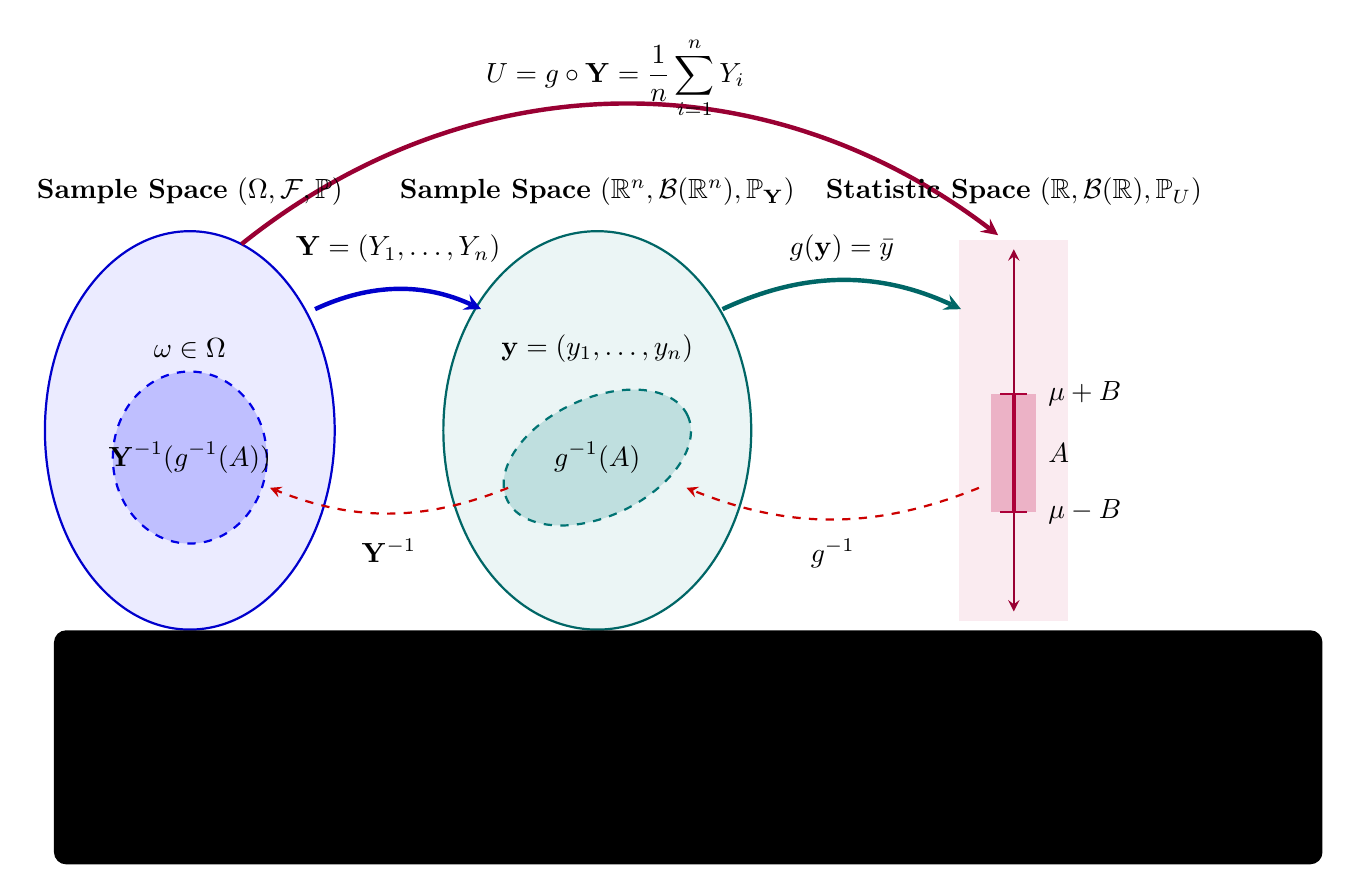
\begin{tikzpicture}[scale=1.15]
    % 1) \fill backgrounds
    \fill[blue!8] (-4.5, 0) ellipse (1.6cm and 2.2cm);
    \fill[blue!25] (-4.5, -0.3) ellipse (0.85cm and 0.95cm);
    
    \fill[teal!8] (0, 0) ellipse (1.7cm and 2.2cm);
    \fill[teal!25, rotate around={25:(0,-0.3)}] (0, -0.3) ellipse (1.1cm and 0.65cm);
    
    \fill[purple!8] (4.0, -2.1) rectangle (5.2, 2.1);
    \fill[purple!30] (4.35, -0.9) rectangle (4.85, 0.4);

    % 2) \draw grid lines / axes / boundaries
    \draw[thick, blue!80!black] (-4.5, 0) ellipse (1.6cm and 2.2cm);
    \draw[thick, dashed, blue!90!black] (-4.5, -0.3) ellipse (0.85cm and 0.95cm);
    
    \draw[thick, teal!80!black] (0, 0) ellipse (1.7cm and 2.2cm);
    \draw[thick, dashed, teal!90!black, rotate around={25:(0,-0.3)}] (0, -0.3) ellipse (1.1cm and 0.65cm);
    
    \draw[thick, purple!80!black, <->, >=stealth] (4.6, -2.0) -- (4.6, 2.0);
    \draw[ultra thick, purple!90!black] (4.6, -0.9) -- (4.6, 0.4);
    \draw[thick, purple!90!black] (4.45, 0.4) -- (4.75, 0.4);
    \draw[thick, purple!90!black] (4.45, -0.9) -- (4.75, -0.9);

    % 3) \draw primary plots / mapping arrows
    % Forward mappings (top)
    \draw[ultra thick, ->, >=stealth, blue!80!black, shorten >=3pt, shorten <=3pt] 
        (-3.2, 1.3) to[bend left=25] (-1.2, 1.3);
    \draw[ultra thick, ->, >=stealth, teal!80!black, shorten >=3pt, shorten <=3pt] 
        (1.3, 1.3) to[bend left=25] (4.1, 1.3);
    \draw[ultra thick, ->, >=stealth, purple!80!black, shorten >=3pt, shorten <=3pt] 
        (-4.0, 2.0) to[bend left=38] (4.5, 2.1);

    % Pre-image pullback arrows (bottom)
    \draw[thick, dashed, ->, >=stealth, red!80!black, shorten >=3pt, shorten <=3pt] 
        (4.3, -0.6) to[bend left=22] (0.9, -0.6);
    \draw[thick, dashed, ->, >=stealth, red!80!black, shorten >=3pt, shorten <=3pt] 
        (-0.9, -0.6) to[bend left=22] (-3.7, -0.6);

    % 4) \node labels/text
    \node[black, above=4pt] at (-4.5, 2.25) {\textbf{Sample Space} $(\Omega, \F, \Prob)$};
    \node[black, above=4pt] at (0, 2.25) {\textbf{Sample Space} $(\R^n, \mathcal{B}(\R^n), \Prob_{\mathbf{Y}})$};
    \node[black, above=4pt] at (4.6, 2.25) {\textbf{Statistic Space} $(\R, \mathcal{B}(\R), \Prob_U)$};

    \node[black] at (-4.5, 0.9) {$\omega \in \Omega$};
    \node[black] at (-4.5, -0.3) {$\displaystyle \mathbf{Y}^{-1}(g^{-1}(A))$};
    
    \node[black] at (0, 0.9) {$\mathbf{y} = (y_1, \dots, y_n)$};
    \node[black] at (0, -0.3) {$\displaystyle g^{-1}(A)$};

    \node[black, right=4pt] at (4.75, 0.4) {$\mu + B$};
    \node[black, right=4pt] at (4.75, -0.9) {$\mu - B$};
    \node[black, right=4pt] at (4.75, -0.25) {$A$};

    % Mapping labels
    \node[black, above=3pt] at (-2.2, 1.65) {$\displaystyle \mathbf{Y} = (Y_1, \dots, Y_n)$};
    \node[black, above=3pt] at (2.7, 1.65) {$\displaystyle g(\mathbf{y}) = \bar{y}$};
    \node[black, above=3pt] at (0.2, 3.25) {$\displaystyle U = g \circ \mathbf{Y} = \frac{1}{n}\sum_{i=1}^{n} Y_i$};

    \node[black, below=3pt] at (2.6, -1.0) {$\displaystyle g^{-1}$};
    \node[black, below=3pt] at (-2.3, -1.0) {$\displaystyle \mathbf{Y}^{-1}$};

    % Single-Node Multiline Legend using Anchor Pivot Strategy
    \node[draw=black, fill=gray!5, thick, rounded corners=4pt, align=left, inner sep=8pt, anchor=west, black] at (-6.0, -3.5) {
        \textbf{Measure-Theoretic Pushforward \& Pre-Image Equivalence:}\\[4pt]
        1. \textbf{Random Sample Mapping:} $\displaystyle \mathbf{Y} : \Omega \to \R^n$ induces joint law $\displaystyle \Prob_{\mathbf{Y}}(E) = \Prob(\mathbf{Y}^{-1}(E))$.\\
        2. \textbf{Estimator Mapping:} $\displaystyle g : \R^n \to \R$ collapses $n$ observations into scalar statistic $\displaystyle U = g(\mathbf{Y})$.\\
        3. \textbf{Sampling Distribution:} $\displaystyle \Prob_U(A) = \Prob(U \in A) = \Prob_{\mathbf{Y}}\left(g^{-1}(A)\right) = \idotsint_{g^{-1}(A)} \prod_{i=1}^{n} f(y_i) \, dy_1 \cdots dy_n$.
    };
\end{tikzpicture}
\end{center}

\vspace{0.4cm}

\begin{center}
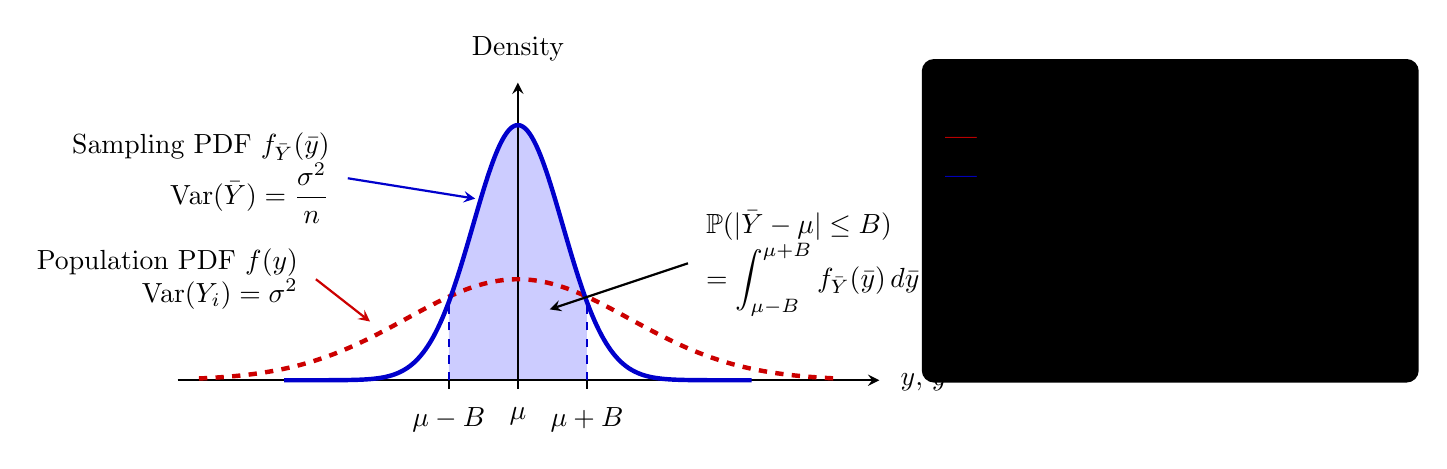
\begin{tikzpicture}[scale=1.35]
    % 1) \fill backgrounds (Shaded Error of Estimation Region under Sampling Distribution of Y-bar)
    \fill[blue!20, domain=-0.65:0.65, smooth, variable=\x] 
        (-0.65, 0) -- plot ({\x}, {2.4*exp(-2.8*\x*\x)}) -- (0.65, 0) -- cycle;

    % 2) \draw grid lines/axes
    \draw[thick, ->, >=stealth] (-3.2, 0) -- (3.4, 0) node[right=4pt, black] {$y, \, \bar{y}$};
    \draw[thick, ->, >=stealth] (0, 0) -- (0, 2.8) node[above=4pt, black] {Density};
    
    % Microscopic tick marks (Decoupled Node Buffers)
    \draw[thick] (0, 0) -- (0, -0.08) node[below=3pt, black] {$\mu$};
    \draw[thick] (-0.65, 0) -- (-0.65, -0.08) node[below=3pt, black] {$\mu - B$};
    \draw[thick] (0.65, 0) -- (0.65, -0.08) node[below=3pt, black] {$\mu + B$};
    \draw[dashed, thick, blue!80!black] (-0.65, 0) -- (-0.65, {2.4*exp(-2.8*0.65*0.65)});
    \draw[dashed, thick, blue!80!black] (0.65, 0) -- (0.65, {2.4*exp(-2.8*0.65*0.65)});

    % 3) \draw primary plots
    % Population density f(y) (wider, variance sigma^2)
    \draw[ultra thick, red!80!black, dashed, domain=-3.0:3.0, samples=100, smooth] 
        plot (\x, {0.95*exp(-0.45*\x*\x)});
        
    % Sampling distribution of Y-bar (narrower, variance sigma^2 / n)
    \draw[ultra thick, blue!80!black, domain=-2.2:2.2, samples=120, smooth] 
        plot (\x, {2.4*exp(-2.8*\x*\x)});

    % Off-axis callout arrows
    \draw[->, >=stealth, thick, shorten >=2pt, blue!80!black] (-1.6, 1.9) -- (-0.35, 1.7);
    \draw[->, >=stealth, thick, shorten >=2pt, red!80!black] (-1.9, 0.95) -- (-1.35, 0.52);
    \draw[->, >=stealth, thick, shorten >=2pt, black] (1.6, 1.1) -- (0.25, 0.65);

    % 4) \node labels/text
    \node[black, left=3pt, align=right] at (-1.6, 1.9) {Sampling PDF $f_{\bar{Y}}(\bar{y})$\\$\displaystyle \text{Var}(\bar{Y}) = \frac{\sigma^2}{n}$};
    \node[black, left=3pt, align=right] at (-1.9, 0.95) {Population PDF $f(y)$\\$\displaystyle \text{Var}(Y_i) = \sigma^2$};
    \node[black, right=3pt, align=left] at (1.6, 1.1) {$\displaystyle \Prob(|\bar{Y} - \mu| \le B)$\\$\displaystyle = \int_{\mu - B}^{\mu + B} f_{\bar{Y}}(\bar{y}) \, d\bar{y}$};

    % Single-Node Multiline Legend using Anchor Pivot Strategy
    \node[draw=black, fill=gray!5, thick, rounded corners=4pt, align=left, inner sep=8pt, anchor=west, black] at (3.8, 1.5) {
        \textbf{Legend \& Asymptotic Behavior:}\\[4pt]
        \textcolor{red!80!black}{\textbf{---}} Population Density $\displaystyle f(y)$\\[2pt]
        \textcolor{blue!80!black}{\textbf{---}} Estimator Density $\displaystyle f_{\bar{Y}}(\bar{y})$\\[4pt]
        As sample size $\displaystyle n \to \infty$:\\
        $\displaystyle \text{Var}(\bar{Y}) = \frac{\sigma^2}{n} \to 0$,\\
        concentrating probability mass\\
        inside $\displaystyle [\mu - B, \mu + B]$.
    };
\end{tikzpicture}
\end{center}

\subsection{Heuristics and ``Cheats'' for Choosing the Optimal Method}

When confronted with a problem asking for the distribution of $U = g(Y_1, \dots, Y_n)$:
\begin{enumerate}[label=\textbf{Heuristic \arabic*:}]
    \item \textbf{Check for Sums of Famous Independent Distributions First (MGF Shortcut):} If $Y_1, \dots, Y_n$ are independent and $U = \sum_{i=1}^n a_i Y_i$ (or $\bar{Y}$), immediately check if $Y_i$ belongs to a family closed under convolution (Normal, Gamma/Exponential/Chi-square with common scale, Poisson, Binomial with common $p$). If so, use \textbf{Method 3 (MGFs)}. A 3-line algebraic product replaces an $n$-dimensional integral!
    \item \textbf{Check for $\min(Y_1, \dots, Y_n)$ or $\max(Y_1, \dots, Y_n)$ (CDF Shortcut):} If $U = \max(Y_1, \dots, Y_n)$, never integrate directly. Use the CDF equivalence $\{ \max_i Y_i \le u \} = \bigcap_{i=1}^n \{Y_i \le u\} \implies F_U(u) = [F_Y(u)]^n$. If $U = \min(Y_1, \dots, Y_n)$, use the survival function $\{ \min_i Y_i > u \} = \bigcap_{i=1}^n \{Y_i > u\} \implies 1 - F_U(u) = [1 - F_Y(u)]^n$.
    \item \textbf{Dimension Matching for Jacobians:} If you have two random variables $(Y_1, Y_2)$ and only want the distribution of a single non-linear combination $U_1 = g(Y_1, Y_2)$ (such as $U_1 = Y_1 / Y_2$ or $U_1 = Y_1 Y_2$), invent a simple auxiliary variable $U_2 = Y_2$ so the mapping $(Y_1, Y_2) \mapsto (U_1, U_2)$ is $\R^2 \to \R^2$ and easily invertible.
\end{enumerate}

\subsection{Common Pitfalls and Logical Fallacies}

\begin{itemize}
    \item \textbf{Pitfall 1: Confusing the Estimator $\bar{Y}$ with the Estimate $\bar{y}$.} Writing $\Prob(|\bar{y} - \mu| \le B) = 0.95$ for a fixed numerical sample average $\bar{y} = 4.2$ is a logical fallacy. Once $\bar{y}$ is realized, $|\bar{y} - \mu| \le B$ is a deterministic proposition that is either true (probability $1$) or false (probability $0$). Randomness resides solely in the random variable estimator $\bar{Y}$ across repeated sampling.
    \item \textbf{Pitfall 2: Forgetting the Absolute Value on the Jacobian.} The area/volume scaling factor in multivariable integration is the \emph{magnitude} $|\det J_{\mathbf{h}^{-1}}(\mathbf{u})|$. Omitting the absolute value bars when $\det J < 0$ yields a negative probability density function—an immediate fatal error.
    \item \textbf{Pitfall 3: Applying the Univariate Transformation Formula to Non-Injective Functions.} If $Y \sim \mathcal{N}(0, 1)$ and $U = Y^2$, blindly writing $f_U(u) = f_Y(\sqrt{u}) \frac{1}{2\sqrt{u}}$ misses half of the probability mass because $y = -\sqrt{u}$ also maps to $u$! For many-to-one mappings, either use the CDF method $F_U(u) = \Prob(-\sqrt{u} \le Y \le \sqrt{u}) = F_Y(\sqrt{u}) - F_Y(-\sqrt{u})$ or partition the domain into strictly monotonic branches and sum over all pre-images:
    \[
        f_U(u) = \sum_{y \in h^{-1}(\{u\})} f_Y(y) \left|\frac{1}{h'(y)}\right|.
    \]
    \item \textbf{Pitfall 4: Assuming Uncorrelated Implies Independent.} While independence guarantees $f(y_1, \dots, y_n) = \prod_{i=1}^n f(y_i)$ and $\text{Cov}(Y_i, Y_j) = 0$, the converse is false in general. Always verify mutual independence before factoring a joint density or multiplying MGFs.
\end{itemize}

\newpage

% ============================================================================
% PART 5: CONCEPTUAL SYNTHESIS AND THE "BIG PICTURE"
% ============================================================================
\section{Conceptual Synthesis and the ``Big Picture''}

\subsection{Thematic Connections}

The unifying mathematical theme of Chapter 6 is the \textbf{Pushforward of Probability Measures under Measurable Mappings}. In earlier chapters of probability theory, a probability distribution is treated as a static object attached to a single random variable $Y$. Section 6.1 reveals that statistical inference is fundamentally dynamic: raw data vectors $\mathbf{Y} \in \R^n$ are transformed through algebraic operators $g : \R^n \to \R^m$ into estimators $\hat{\theta} = g(\mathbf{Y})$, test statistics $T = g(\mathbf{Y})$, and empirical loss functions.

This theme unifies three major pillars of mathematics:
\begin{enumerate}[label=\arabic*.]
    \item \textbf{Measure Theory:} Preservation of measurability under function composition ($U = g \circ \mathbf{Y}$) and the Change-of-Variables Formula for pushforward integrals:
    \[
        \E[u(g(\mathbf{Y}))] = \int_{\Omega} u(g(\mathbf{Y}(\omega))) \, d\Prob(\omega) = \int_{\R^n} u(g(\mathbf{y})) \, d\Prob_{\mathbf{Y}}(\mathbf{y}) = \int_{\R} u(z) \, d\Prob_U(z).
    \]
    \item \textbf{Harmonic and Complex Analysis:} The Method of Moment-Generating Functions (and Characteristic Functions $\varphi_{\mathbf{Y}}(t) = \E[e^{itY}]$) is simply the Laplace/Fourier transform of a measure, converting the analytic operation of measure convolution ($\Prob_{Y_1 + Y_2} = \Prob_{Y_1} * \Prob_{Y_2}$) into pointwise multiplication of functions in the frequency domain.
    \item \textbf{Differential Geometry:} The Method of Jacobians treats $(Y_1, \dots, Y_n)$ as coordinates on a smooth manifold and pulls back the volume form $f_{\mathbf{Y}}(\mathbf{y}) \, dy_1 \wedge \cdots \wedge dy_n$ along a diffeomorphism $\mathbf{h}^{-1}$.
\end{enumerate}

\subsection{Forward and Backward Links}

\begin{itemize}
    \item \textbf{Backward Links (Foundations Built Upon):}
    \begin{itemize}
        \item \emph{Combinatorics and Finite Probability (Chapter 2 \& 3):} Random sampling without replacement (Hypergeometric trials) provides the finite-population baseline whose $N \to \infty$ limit justifies the i.i.d. product measure $p(y_1, \dots, y_n) = \prod_{i=1}^n p(y_i)$ in Section 6.1.
        \item \emph{Multivariate Distributions and Independence (Chapter 5):} Marginalization, conditional densities, and expectation of multivariate functions provide the integration mechanics required to execute the CDF and Jacobian methods.
    \end{itemize}
    \item \textbf{Forward Links (Bedrock for Advanced Topics):}
    \begin{itemize}
        \item \emph{Sampling Distributions and the Central Limit Theorem (Chapter 7):} Using the MGF method of Section 6.2/6.5 on the standardized sample mean $Z_n = \frac{\bar{Y} - \mu}{\sigma/\sqrt{n}}$ proves that $\lim_{n \to \infty} M_{Z_n}(t) = e^{t^2/2}$ (the Central Limit Theorem), as well as Cochran's Theorem and the exact $\chi^2_{n-1}$, Student's $t$, and $F$ distributions for normal samples.
        \item \emph{Point and Interval Estimation (Chapters 8 \& 9):} The quantity $\Prob(|\bar{Y} - \mu| \le B) = 1 - \alpha$ introduced in Section 6.1 is literally the algebraic inversion that constructs a $100(1-\alpha)\%$ Confidence Interval $[\bar{Y} - B, \bar{Y} + B]$ and defines Consistency ($\bar{Y} \xrightarrow{\Prob} \mu$), Efficiency, and Rao-Blackwell sufficiency reductions.
        \item \emph{Stochastic Calculus and Quantitative Finance:} Extending functions of finitely many random variables $g(Y_1, \dots, Y_n)$ to functions of continuous-time stochastic processes $g(t, W_t)$ leads directly to \textbf{It\^o's Lemma}, the stochastic generalization of the transformation rule.
    \end{itemize}
\end{itemize}

\newpage

% ============================================================================
% PART 6: ABSTRACT REAL-WORLD MODELING (AI, ML, & QUANT FINANCE)
% ============================================================================
\section{Abstract Real-World Modeling in AI, Machine Learning, and Quantitative Finance}

\subsection{Concrete Advanced Scenarios}

\begin{enumerate}[label=\textbf{Scenario \arabic*:}]
    \item \textbf{Generative AI — Normalizing Flows and Invertible Neural Networks (Method of Jacobians):} \\ \relax
    In modern generative modeling (e.g., RealNVP, Glow, Continuous Normalizing Flows), an AI system must learn to sample complex, high-dimensional data distributions $\mathbf{X} \in \R^d$ (such as photorealistic images or molecular conformations). The model starts with an i.i.d. random sample $\mathbf{Z} = (Z_1, \dots, Z_d)^T \sim \mathcal{N}(\mathbf{0}, I_d)$ from a simple isotropic Gaussian base distribution with factored joint density $f_{\mathbf{Z}}(\mathbf{z}) = \prod_{i=1}^d \phi(z_i)$, and passes $\mathbf{Z}$ through a composition of parameterized bijective neural network layers $\mathbf{X} = \mathbf{g}_{\theta}(\mathbf{Z}) = \mathbf{g}_K \circ \cdots \circ \mathbf{g}_1(\mathbf{Z})$. The exact log-likelihood of training data is computed directly via Section 6.2's Multivariable Jacobian Theorem:
    \[
        \log f_{\mathbf{X}}(\mathbf{x}; \theta) = \sum_{i=1}^{d} \log \phi\left(\left(\mathbf{g}_{\theta}^{-1}(\mathbf{x})\right)_i\right) + \sum_{k=1}^{K} \log \left|\det J_{\mathbf{g}_k^{-1}}\right|.
    \]

    \item \textbf{Statistical Learning Theory — Empirical Risk Minimization and PAC Generalization Bounds (Error of Estimation of Sample Means):} \\ \relax
    In supervised Machine Learning, we observe an i.i.d. training dataset $S = \{Z_1, \dots, Z_n\}$ where $Z_i = (X_i, Y_i) \stackrel{\text{i.i.d.}}{\sim} \Prob_Z$. For a neural network or classifier parameterized by weights $w \in \mathcal{W}$ with loss function $\ell(w, Z_i)$, the true population risk is $\mu(w) = R(w) \coloneqq \E[\ell(w, Z)]$, while the training algorithm minimizes the \emph{empirical risk}—which is precisely the sample mean of functions of random variables:
    \[
        \bar{Y}_n(w) = \hat{R}_n(w) \coloneqq \frac{1}{n} \sum_{i=1}^{n} \ell(w, Z_i).
    \]
    Determining the probability that the generalization error $|\hat{R}_n(w) - R(w)|$ is at most $B = \epsilon$ (via Hoeffding's Inequality, McDiarmid's Inequality, and Rademacher Complexity) is the exact high-dimensional machine learning analog of Section 6.1's error of estimation $\Prob(|\bar{Y} - \mu| \le B)$.

    \item \textbf{Quantitative Finance — Multi-Asset Derivative Pricing and Portfolio Value-at-Risk (Functions of Random Vectors \& Stochastic Calculus):} \\ \relax
    A quantitative trading desk holds a portfolio of $n$ risky assets whose log-returns $(Y_1, \dots, Y_n)$ over horizon $T$ follow a joint distribution $f(y_1, \dots, y_n)$. The terminal portfolio value or basket option payoff is a non-linear function $U = g(Y_1, \dots, Y_n) = \max\left(\sum_{i=1}^n w_i S_i(0)e^{Y_i} - K, 0\right)$. Deriving the distribution $F_U(u)$ of $U$ is required both to price the derivative under the risk-neutral measure $\mathbb{Q}$ and to compute the regulatory Value-at-Risk $\text{VaR}_{\alpha}(U) = \inf\{u \in \R : F_U(u) \ge \alpha\}$.
\end{enumerate}

\subsection{Rigorous Mathematical Model Setup: Normalizing Flow Coupled with It\^o Diffusion for Quantitative Asset Pricing}

Let us formulate a research-grade mathematical model combining **Scenario 1** (Invertible Neural Network Jacobian Flows) and **Scenario 3** (Stochastic Calculus Derivative Pricing and Monte Carlo Sample Mean Estimation).

\subsubsection*{1. Filtered Probability Space and Continuous-Time It\^o Dynamics}
Let $(\Omega, \F, \{\F_t\}_{t \ge 0}, \mathbb{Q})$ be a complete filtered probability space supporting a $d$-dimensional standard Brownian motion $\mathbf{W}_t = (W_t^{(1)}, \dots, W_t^{(d)})^T$ under the risk-neutral measure $\mathbb{Q}$. Consider $d$ underlying financial assets $\mathbf{S}_t = (S_t^{(1)}, \dots, S_t^{(d)})^T$ governed by the system of stochastic differential equations:
\[
    dS_t^{(i)} = r S_t^{(i)} \, dt + S_t^{(i)} \sum_{j=1}^{d} \sigma_{ij} \, dW_t^{(j)}, \qquad S_0^{(i)} > 0, \quad i = 1, \dots, d,
\]
where $r > 0$ is the constant risk-free interest rate and $\Sigma = (\sigma_{ij}) \in \R^{d \times d}$ is a non-singular volatility matrix with covariance matrix $C = \Sigma \Sigma^T$.

Applying \textbf{It\^o's Lemma} (the continuous-time stochastic transformation rule) to the logarithmic transformation $X_t^{(i)} = h(S_t^{(i)}) = \log S_t^{(i)}$, since $\frac{\partial h}{\partial s} = \frac{1}{s}$ and $\frac{\partial^2 h}{\partial s^2} = -\frac{1}{s^2}$, we obtain:
\begin{align*}
    dX_t^{(i)} &= \frac{1}{S_t^{(i)}} \, dS_t^{(i)} - \frac{1}{2\left(S_t^{(i)}\right)^2} \, d\langle S^{(i)}, S^{(i)} \rangle_t \\ \relax
    &= \left(r - \frac{1}{2} C_{ii}\right) dt + \sum_{j=1}^{d} \sigma_{ij} \, dW_t^{(j)}.
\end{align*}
Integrating from $t = 0$ to maturity $T > 0$ shows that the terminal log-price vector $\mathbf{X}_T = \mathbf{h}_{\text{It\^o}}(\mathbf{Z})$ is an affine transformation of an i.i.d. standard normal random sample $\mathbf{Z} = (Z_1, \dots, Z_d)^T \sim \mathcal{N}(\mathbf{0}, I_d)$:
\[
    \mathbf{X}_T = \boldsymbol{\mu}_T + \sqrt{T} \Sigma \mathbf{Z}, \qquad \text{where } \mu_T^{(i)} = \log S_0^{(i)} + \left(r - \frac{1}{2}C_{ii}\right)T.
\]

\subsubsection*{2. Non-Gaussian Tail Calibration via Deep Diffeomorphic Jacobian Flow}
To capture empirical heavy tails and implied volatility skew beyond log-normality, we pass $\mathbf{X}_T$ through a parameterized $K$-layer diffeomorphic normalizing flow $\mathbf{g}_{\theta} : \R^d \to \R^d_+$, setting the terminal asset prices to $\mathbf{S}_T = \mathbf{g}_{\theta}(\mathbf{X}_T)$. By the **Multivariable Jacobian Method (Section 6.2 / 6.6)** and the chain rule for determinants, the exact risk-neutral joint density $f_{\mathbf{S}_T}^{\mathbb{Q}}(\mathbf{s}; \theta)$ on $\R^d_+$ is:
\[
    f_{\mathbf{S}_T}^{\mathbb{Q}}(\mathbf{s}; \theta) = \frac{1}{(2\pi T)^{d/2} |\det \Sigma|} \exp\left( -\frac{1}{2T} \left(\mathbf{g}_{\theta}^{-1}(\mathbf{s}) - \boldsymbol{\mu}_T\right)^T C^{-1} \left(\mathbf{g}_{\theta}^{-1}(\mathbf{s}) - \boldsymbol{\mu}_T\right) \right) \left|\det J_{\mathbf{g}_{\theta}^{-1}}(\mathbf{s})\right|.
\]

\subsubsection*{3. Monte Carlo Sample Mean Estimator and Optimization Problem}
Let $\Psi : \R^d_+ \to [0, \infty)$ be a multi-asset contingent claim payoff function (e.g., an arithmetic basket call $\Psi(\mathbf{S}_T) = \max\left(\frac{1}{d}\sum_{i=1}^d S_T^{(i)} - K, 0\right)$). The arbitrage-free price of the derivative at $t = 0$ is the population mean $\mu_{\theta} = \E^{\mathbb{Q}}\left[e^{-rT}\Psi(\mathbf{S}_T)\right]$. Drawing $n$ i.i.d. base vectors $\mathbf{Z}^{(1)}, \dots, \mathbf{Z}^{(n)} \stackrel{\text{i.i.d.}}{\sim} \mathcal{N}(\mathbf{0}, I_d)$, we define the i.i.d. discounted payoff random variables
\[
    Y_m(\theta) \coloneqq e^{-rT} \Psi\left( \mathbf{g}_{\theta}\left(\boldsymbol{\mu}_T + \sqrt{T}\Sigma \mathbf{Z}^{(m)}\right) \right), \qquad m = 1, \dots, n,
\]
and estimate $\mu_{\theta}$ via the Section 6.1 sample mean estimator:
\[
    \bar{Y}_n(\theta) = \frac{1}{n} \sum_{m=1}^{n} Y_m(\theta).
\]
To calibrate the flow parameters $\theta \in \Theta$ to $M$ observed market option prices $\{V_j^{\text{mkt}}\}_{j=1}^M$ while guaranteeing that the Monte Carlo error of estimation satisfies $\mathbb{Q}\left(|\bar{Y}_n(\theta) - \mu_{\theta}| \le B\right) \ge 1 - \alpha$, the quantitative researcher solves the constrained stochastic optimization problem:
\[
    \min_{\theta \in \Theta} \mathcal{L}(\theta) \coloneqq \sum_{j=1}^{M} w_j \left( \frac{1}{n} \sum_{m=1}^{n} e^{-rT} \Psi_j\left(\mathbf{g}_{\theta}(\mathbf{X}_T^{(m)})\right) - V_j^{\text{mkt}} \right)^2 + \lambda \|\theta\|_2^2 \quad \text{subject to} \quad n \ge \frac{\text{Var}^{\mathbb{Q}}(Y_m(\theta))}{\alpha B^2}.
\]

\newpage

% ============================================================================
% PART 7: COMMON VARIATIONS AND UNTESTED CONCEPTS
% ============================================================================
\section{Common Variations and Untested Concepts}

Because Sections 6.1 and 6.2 serve as the conceptual gateway to Chapter 6, university examinations routinely test three major operational extensions that are previewed in Section 6.2 but not explicitly worked out in the introductory text. Below, we state and rigorously prove each of these essential variations.

\subsection{Variation 1: Non-Monotonic (Many-to-One) Transformations and the Chi-Square ($\chi^2_1$) Law}

\begin{proposition}[Distribution of $U = Y^2$ for Standard Normal $Y$]
Let $Y \sim \mathcal{N}(0, 1)$ have standard normal density $f_Y(y) = \frac{1}{\sqrt{2\pi}} e^{-y^2/2}$ for $y \in \R$. Prove that the non-monotonic function $U = g(Y) = Y^2$ follows a $\chi^2(1)$ (Chi-square with $1$ degree of freedom) distribution, i.e., $\text{Gamma}(\alpha = 1/2, \beta = 2)$.
\end{proposition}

\begin{proof}
Since $Y^2 \ge 0$ for all $y \in \R$, $F_U(u) = \Prob(Y^2 \le u) = 0$ for $u \le 0$. For any $u > 0$, the mapping $y \mapsto y^2$ is two-to-one on $\R \setminus \{0\}$, with pre-image interval $\{y \in \R : y^2 \le u\} = [-\sqrt{u}, \sqrt{u}]$. Using the Method of Distribution Functions (Method 1):
\[
    F_U(u) = \Prob(Y^2 \le u) = \Prob\left(-\sqrt{u} \le Y \le \sqrt{u}\right) = F_Y\left(\sqrt{u}\right) - F_Y\left(-\sqrt{u}\right).
\]
Differentiating both sides with respect to $u > 0$ via the Fundamental Theorem of Calculus and the Chain Rule:
\begin{align*}
    f_U(u) &= \frac{d}{du} F_U(u) = f_Y\left(\sqrt{u}\right) \frac{d}{du}\left(\sqrt{u}\right) - f_Y\left(-\sqrt{u}\right) \frac{d}{du}\left(-\sqrt{u}\right) \\ \relax
    &= f_Y\left(\sqrt{u}\right) \left(\frac{1}{2\sqrt{u}}\right) - f_Y\left(-\sqrt{u}\right) \left(-\frac{1}{2\sqrt{u}}\right) \\ \relax
    &= \frac{1}{2\sqrt{u}} \left[ f_Y\left(\sqrt{u}\right) + f_Y\left(-\sqrt{u}\right) \right].
\end{align*}
Substituting $f_Y(\pm\sqrt{u}) = \frac{1}{\sqrt{2\pi}} e^{-(\pm\sqrt{u})^2/2} = \frac{1}{\sqrt{2\pi}} e^{-u/2}$ and recalling that $\Gamma(1/2) = \sqrt{\pi}$:
\[
    f_U(u) = \frac{1}{2\sqrt{u}} \left( \frac{2}{\sqrt{2\pi}} e^{-u/2} \right) = \frac{1}{\sqrt{\pi} \, 2^{1/2}} u^{1/2 - 1} e^{-u/2} = \frac{1}{\Gamma(1/2) \, 2^{1/2}} u^{1/2 - 1} e^{-u/2} \mathbf{1}_{(0, \infty)}(u).
\]
This is precisely the PDF of $\text{Gamma}(\alpha = 1/2, \beta = 2) \equiv \chi^2(1)$. Moreover, if $Y_1, \dots, Y_n \stackrel{\text{i.i.d.}}{\sim} \mathcal{N}(0, 1)$, then by the MGF method, $\sum_{i=1}^n Y_i^2 \sim \prod_{i=1}^n (1 - 2t)^{-1/2} = (1 - 2t)^{-n/2} \equiv \chi^2(n)$.
\end{proof}

\subsection{Variation 2: The Convolution Integral for the Sum of Independent Random Variables}

\begin{proposition}[General Convolution Formula]
Let $Y_1$ and $Y_2$ be independent continuous random variables with marginal densities $f_{Y_1}(y_1)$ and $f_{Y_2}(y_2)$. Prove that the density of their sum $U = Y_1 + Y_2$ is given by the convolution integral
\[
    f_U(u) = (f_{Y_1} * f_{Y_2})(u) \coloneqq \int_{-\infty}^{\infty} f_{Y_1}(u - y_2) f_{Y_2}(y_2) \, dy_2.
\]
\end{proposition}

\begin{proof}
Define the invertible linear mapping $(U_1, U_2) = (Y_1 + Y_2, Y_2)$ on $\R^2$, which has inverse $y_1 = u_1 - u_2$ and $y_2 = u_2$. The Jacobian determinant is
\[
    \det J = \begin{vmatrix} 1 & -1 \\ 0 & 1 \end{vmatrix} = 1.
\]
By independence, $f_{Y_1, Y_2}(y_1, y_2) = f_{Y_1}(y_1)f_{Y_2}(y_2)$, so the joint PDF of $(U_1, U_2)$ is $f_{U_1, U_2}(u_1, u_2) = f_{Y_1}(u_1 - u_2)f_{Y_2}(u_2)$. Integrating out $u_2 \in (-\infty, \infty)$ gives the marginal PDF of $U = U_1$:
\[
    f_U(u) = \int_{-\infty}^{\infty} f_{Y_1}(u - u_2) f_{Y_2}(u_2) \, du_2.
\]
\end{proof}

\subsection{Variation 3: Exact Distribution of the Extreme Order Statistics ($Y_{(1)}$ and $Y_{(n)}$)}

\begin{proposition}[Order Statistics of an I.I.D. Sample — Section 6.7 Preview]
Let $Y_1, Y_2, \dots, Y_n$ be an i.i.d. random sample from a continuous population with CDF $F(y)$ and PDF $f(y)$. Let $Y_{(1)} = \min(Y_1, \dots, Y_n)$ and $Y_{(n)} = \max(Y_1, \dots, Y_n)$. Prove that:
\[
    f_{Y_{(n)}}(y) = n \left[F(y)\right]^{n-1} f(y), \qquad f_{Y_{(1)}}(y) = n \left[1 - F(y)\right]^{n-1} f(y).
\]
\end{proposition}

\begin{proof}
For the maximum $Y_{(n)}$, note that the maximum of $n$ numbers is at most $y$ if and only if \emph{every single} number is at most $y$:
\[
    F_{Y_{(n)}}(y) = \Prob\left(\max_{1 \le i \le n} Y_i \le y\right) = \Prob\left(\bigcap_{i=1}^{n} \{Y_i \le y\}\right) = \prod_{i=1}^{n} \Prob(Y_i \le y) = \left[F(y)\right]^n,
\]
where the third equality follows from mutual independence and the fourth from identical distribution. Differentiating with respect to $y$ via the chain rule yields $f_{Y_{(n)}}(y) = n [F(y)]^{n-1} f(y)$.

Similarly, for the minimum $Y_{(1)}$, the minimum of $n$ numbers is strictly greater than $y$ if and only if \emph{every single} number is strictly greater than $y$:
\[
    F_{Y_{(1)}}(y) = 1 - \Prob\left(\min_{1 \le i \le n} Y_i > y\right) = 1 - \Prob\left(\bigcap_{i=1}^{n} \{Y_i > y\}\right) = 1 - \prod_{i=1}^{n} \Prob(Y_i > y) = 1 - \left[1 - F(y)\right]^n.
\]
Differentiating with respect to $y$ gives $f_{Y_{(1)}}(y) = -n [1 - F(y)]^{n-1} (-f(y)) = n [1 - F(y)]^{n-1} f(y)$.
\end{proof}

\newpage

% ============================================================================
% PART 8: ADVANCED DIAGNOSTIC TESTING: "FIND THE FLAW"
% ============================================================================
\section{Advanced Diagnostic Testing: ``Find the Flaw''}

Below are five complete, seemingly rigorous mathematical proofs and solutions related to Sections 6.1 and 6.2. Each proof contains \textbf{one fatal logical, analytical, or measure-theoretic flaw}. Act as the grader: identify the exact line where the error occurs, explain why it is invalid, and provide the corrected derivation before consulting the Solution Key in Section 8.2.

\subsection{The Five Flawed Proofs}

\subsubsection*{Diagnostic Problem 1: The Cauchy Sample Mean Paradox}
\textbf{Claim:} Let $Y_1, \dots, Y_n$ be an i.i.d. random sample from a standard Cauchy population with density $f(y) = \frac{1}{\pi(1 + y^2)}$ for $y \in \R$. As $n \to \infty$, the error of estimation $|\bar{Y} - 0|$ converges in probability to $0$, i.e., $\lim_{n \to \infty} \Prob(|\bar{Y}| \le B) = 1$ for any $B > 0$.

\textbf{Proposed ``Proof'':}
\begin{enumerate}[label=\textbf{Line \arabic*:}]
    \item By definition of the Cauchy density, $f(-y) = \frac{1}{\pi(1 + (-y)^2)} = \frac{1}{\pi(1 + y^2)} = f(y)$, so $f(y)$ is symmetric around $0$.
    \item By symmetry, the population mean is $\mu = \int_{-\infty}^{\infty} y f(y) \, dy = 0$.
    \item For an i.i.d. sample $Y_1, \dots, Y_n$, the sample mean $\bar{Y} = \frac{1}{n}\sum_{i=1}^n Y_i$ has expectation $\E[\bar{Y}] = \mu = 0$ and variance $\text{Var}(\bar{Y}) = \frac{\sigma^2}{n}$.
    \item By Chebyshev's Inequality for any $B > 0$, $\Prob(|\bar{Y} - 0| \le B) \ge 1 - \frac{\sigma^2}{n B^2}$.
    \item Taking the limit as $n \to \infty$ gives $\lim_{n \to \infty} \Prob(|\bar{Y}| \le B) \ge 1 - 0 = 1$, proving $\Prob(|\bar{Y}| \le B) \to 1$. \hfill $\square$
\end{enumerate}

---

\subsubsection*{Diagnostic Problem 2: Joint Density Factorization Under Zero Covariance}
\textbf{Claim:} Let $Y_1 \sim \mathcal{N}(0, 1)$ and define $Y_2 = W Y_1$, where $W \in \{-1, 1\}$ is a Rademacher random variable ($\Prob(W = 1) = \Prob(W = -1) = 1/2$) independent of $Y_1$. Then the sample mean $\bar{Y} = \frac{Y_1 + Y_2}{2}$ has a $\mathcal{N}(0, 1/2)$ distribution.

\textbf{Proposed ``Proof'':}
\begin{enumerate}[label=\textbf{Line \arabic*:}]
    \item First, verify the marginal distribution of $Y_2$: for any $y \in \R$, $\Prob(Y_2 \le y) = \frac{1}{2}\Prob(Y_1 \le y) + \frac{1}{2}\Prob(-Y_1 \le y) = \frac{1}{2}\Phi(y) + \frac{1}{2}\Phi(y) = \Phi(y)$, so $Y_2 \sim \mathcal{N}(0, 1)$.
    \item Next, compute the covariance between $Y_1$ and $Y_2$: $\text{Cov}(Y_1, Y_2) = \E[Y_1 Y_2] - \E[Y_1]\E[Y_2] = \E[W Y_1^2] - 0 = \E[W]\E[Y_1^2] = 0 \cdot 1 = 0$.
    \item Because $Y_1$ and $Y_2$ are normally distributed and uncorrelated ($\text{Cov}(Y_1, Y_2) = 0$), $Y_1$ and $Y_2$ are mutually independent with joint density $f(y_1, y_2) = f(y_1)f(y_2)$.
    \item Applying the Method of Moment-Generating Functions to $\bar{Y} = \frac{1}{2}Y_1 + \frac{1}{2}Y_2$:
    \[
        M_{\bar{Y}}(t) = M_{Y_1}(t/2) M_{Y_2}(t/2) = e^{t^2/8} e^{t^2/8} = e^{t^2/4}.
    \]
    \item By MGF uniqueness, $\bar{Y} \sim \mathcal{N}(0, 1/2)$. \hfill $\square$
\end{enumerate}

---

\subsubsection*{Diagnostic Problem 3: Univariate Transformation of a Symmetric Domain}
\textbf{Claim:} Let $Y \sim \text{Uniform}(-1, 2)$ have density $f_Y(y) = \frac{1}{3}$ for $-1 < y < 2$ and $0$ otherwise. Then $U = Y^2$ has density $f_U(u) = \frac{1}{3\sqrt{u}}$ for $0 < u < 4$.

\textbf{Proposed ``Proof'':}
\begin{enumerate}[label=\textbf{Line \arabic*:}]
    \item Since $y \in (-1, 2)$, the range of $U = Y^2$ is $u \in [0, 4)$.
    \item For any $u \in (0, 4)$, the equation $y^2 = u$ has two real roots: $y_1 = \sqrt{u}$ and $y_2 = -\sqrt{u}$.
    \item The Jacobian derivatives of the two inverse branches are $\left|\frac{dy_1}{du}\right| = \frac{1}{2\sqrt{u}}$ and $\left|\frac{dy_2}{du}\right| = \frac{1}{2\sqrt{u}}$.
    \item Summing over both branches for all $u \in (0, 4)$ gives:
    \[
        f_U(u) = f_Y(\sqrt{u})\frac{1}{2\sqrt{u}} + f_Y(-\sqrt{u})\frac{1}{2\sqrt{u}} = \frac{1}{3}\frac{1}{2\sqrt{u}} + \frac{1}{3}\frac{1}{2\sqrt{u}} = \frac{1}{3\sqrt{u}}, \quad 0 < u < 4.
    \]
    \hfill $\square$
\end{enumerate}

---

\subsubsection*{Diagnostic Problem 4: Bivariate Jacobian Integration Limits}
\textbf{Claim:} Let $Y_1, Y_2 \stackrel{\text{i.i.d.}}{\sim} \text{Uniform}(0, 1)$ with joint density $f(y_1, y_2) = 1$ on $(0, 1)^2$. Then the sum $U_1 = Y_1 + Y_2$ has a $\text{Uniform}(0, 2)$ distribution with density $f_{U_1}(u_1) = 1$ for $0 < u_1 < 2$.

\textbf{Proposed ``Proof'':}
\begin{enumerate}[label=\textbf{Line \arabic*:}]
    \item Define the transformation $U_1 = Y_1 + Y_2$ and $U_2 = Y_2$, with inverse $y_1 = u_1 - u_2$ and $y_2 = u_2$.
    \item The Jacobian determinant is $\det J = \begin{vmatrix} 1 & -1 \\ 0 & 1 \end{vmatrix} = 1$.
    \item Since $0 < y_1 < 1$ and $0 < y_2 < 1$, the range of $U_1 = Y_1 + Y_2$ is $0 < u_1 < 2$ and the range of $U_2 = Y_2$ is $0 < u_2 < 1$.
    \item Substituting into the Jacobian formula gives $f_{U_1, U_2}(u_1, u_2) = 1 \cdot |1| = 1$ for $0 < u_1 < 2$ and $0 < u_2 < 1$.
    \item Integrating out $u_2$ over its support $(0, 1)$ yields $f_{U_1}(u_1) = \int_{0}^{1} 1 \, du_2 = 1$ for $0 < u_1 < 2$. \hfill $\square$
\end{enumerate}

---

\subsubsection*{Diagnostic Problem 5: Finite Population Variance of the Sample Mean}
\textbf{Claim:} Suppose we draw a random sample $Y_1, \dots, Y_n$ of size $n = 50$ \emph{without replacement} from a finite population of size $N = 100$ with population mean $\mu$ and variance $\sigma^2$. Then $\text{Var}(\bar{Y}) = \frac{\sigma^2}{50}$.

\textbf{Proposed ``Proof'':}
\begin{enumerate}[label=\textbf{Line \arabic*:}]
    \item By exchangeability of simple random sampling without replacement, each observation $Y_i$ ($i = 1, \dots, n$) has marginal mean $\E[Y_i] = \mu$ and marginal variance $\text{Var}(Y_i) = \sigma^2$.
    \item By linearity of expectation, $\E[\bar{Y}] = \frac{1}{n}\sum_{i=1}^n \E[Y_i] = \mu$.
    \item Applying the variance operator to $\bar{Y} = \frac{1}{n}\sum_{i=1}^n Y_i$ gives:
    \[
        \text{Var}(\bar{Y}) = \text{Var}\left(\frac{1}{n}\sum_{i=1}^{n} Y_i\right) = \frac{1}{n^2} \sum_{i=1}^{n} \text{Var}(Y_i) = \frac{n\sigma^2}{n^2} = \frac{\sigma^2}{n} = \frac{\sigma^2}{50}.
    \]
    \hfill $\square$
\end{enumerate}

\newpage

\subsection{Solution Key and Rigorous Resolutions}

\begin{enumerate}[label=\textbf{Resolution \arabic*:}]
    \item \textbf{Diagnostic Problem 1 (Cauchy Sample Mean Paradox):}
    \begin{itemize}
        \item \emph{Location of Flaw:} \textbf{Lines 2 and 3.}
        \item \emph{Why It Is an Error:} In Lebesgue integration, a function $g(y) = y f(y)$ is integrable ($\E[|Y|] < \infty$) if and only if $\int_{-\infty}^{\infty} |y| f(y) \, dy < \infty$. For the Cauchy distribution,
        \[
            \int_{-\infty}^{\infty} \frac{|y|}{\pi(1 + y^2)} \, dy = \frac{2}{\pi} \lim_{M \to \infty} \left[ \frac{1}{2} \ln(1 + y^2) \right]_{0}^{M} = \infty.
        \]
        The Cauchy distribution has \textbf{no mean} ($\mu$ does not exist; only the Cauchy principal value is $0$) and \textbf{infinite variance} ($\sigma^2 = \infty$). Therefore, $\text{Var}(\bar{Y}) = \sigma^2/n$ and Chebyshev's Inequality are completely inapplicable!
        \item \emph{Correct Mathematical Step:} Using the Characteristic Function $\varphi_{Y_i}(t) = \E[e^{itY_i}] = e^{-|t|}$, the characteristic function of the sample mean $\bar{Y}$ is $\varphi_{\bar{Y}}(t) = \prod_{i=1}^n \varphi_{Y_i}(t/n) = \prod_{i=1}^n e^{-|t|/n} = e^{-|t|}$. Remarkably, $\bar{Y} \sim \text{Cauchy}(0, 1)$ for \emph{every} $n \ge 1$! Increasing the sample size $n$ does not reduce the error of estimation at all: $\Prob(|\bar{Y}| \le B) = \frac{2}{\pi}\arctan(B) < 1$ is constant for all $n$.
    \end{itemize}

    \item \textbf{Diagnostic Problem 2 (Zero Covariance vs. Joint Normality):}
    \begin{itemize}
        \item \emph{Location of Flaw:} \textbf{Line 3.}
        \item \emph{Why It Is an Error:} While it is true that \emph{jointly normal} uncorrelated random variables are independent, $Y_1$ and $Y_2 = W Y_1$ are only \emph{marginally} normal, NOT jointly (bivariate) normal! In fact, $|Y_2| = |Y_1|$ with probability $1$, so they are maximally dependent ($Y_1^2 = Y_2^2$), and their joint distribution is supported entirely on the two diagonals $y_2 = y_1$ and $y_2 = -y_1$ in $\R^2$. Thus $f(y_1, y_2) \neq f(y_1)f(y_2)$ and $M_{\bar{Y}}(t) \neq M_{Y_1}(t/2)M_{Y_2}(t/2)$.
        \item \emph{Correct Mathematical Step:} Conditioning on $W$: with probability $1/2$, $W = -1 \implies \bar{Y} = \frac{Y_1 - Y_1}{2} = 0$; with probability $1/2$, $W = +1 \implies \bar{Y} = \frac{Y_1 + Y_1}{2} = Y_1 \sim \mathcal{N}(0, 1)$. Thus $\bar{Y}$ is a mixed discrete-continuous distribution with a point mass of $1/2$ at $0$ and a Gaussian density $\frac{1}{2}\phi(y)$ elsewhere.
    \end{itemize}

    \item \textbf{Diagnostic Problem 3 (Asymmetric Domain Pre-Image Error):}
    \begin{itemize}
        \item \emph{Location of Flaw:} \textbf{Line 4.}
        \item \emph{Why It Is an Error:} The author assumed $f_Y(-\sqrt{u}) = 1/3$ for all $u \in (0, 4)$. However, the support of $Y$ is $(-1, 2)$. When $u \in (1, 4)$, the negative root is $-\sqrt{u} \in (-2, -1)$, which lies \emph{outside} the support of $Y$, so $f_Y(-\sqrt{u}) = 0$ for $1 < u < 4$! (Notice that integrating the flawed density gives $\int_0^4 \frac{1}{3\sqrt{u}}\,du = \frac{4}{3} \neq 1$.)
        \item \emph{Correct Mathematical Step:} Partition the range of $U$ into two regimes:
        \begin{itemize}
            \item For $0 < u < 1$: Both $\sqrt{u} \in (0, 1) \subset (-1, 2)$ and $-\sqrt{u} \in (-1, 0) \subset (-1, 2)$ are active, so $f_U(u) = \frac{1}{3}\frac{1}{2\sqrt{u}} + \frac{1}{3}\frac{1}{2\sqrt{u}} = \frac{1}{3\sqrt{u}}$.
            \item For $1 \le u < 4$: Only the positive branch $\sqrt{u} \in [1, 2) \subset (-1, 2)$ is active ($f_Y(-\sqrt{u}) = 0$), so $f_U(u) = \frac{1}{3}\frac{1}{2\sqrt{u}} + 0 = \frac{1}{6\sqrt{u}}$.
        \end{itemize}
        Now $\int_0^1 \frac{1}{3\sqrt{u}}\,du + \int_1^4 \frac{1}{6\sqrt{u}}\,du = \frac{2}{3} + \frac{1}{3} = 1$.
    \end{itemize}

    \item \textbf{Diagnostic Problem 4 (Coupled Support Constraints in Jacobians):}
    \begin{itemize}
        \item \emph{Location of Flaw:} \textbf{Lines 3, 4, and 5.}
        \item \emph{Why It Is an Error:} The inequalities $0 < y_1 < 1$ and $0 < y_2 < 1$ translate under the inverse map $y_1 = u_1 - u_2, \, y_2 = u_2$ into $0 < u_1 - u_2 < 1$ and $0 < u_2 < 1$. The first inequality requires $u_1 - 1 < u_2 < u_1$. Thus the transformed region $\mathcal{T}$ is a parallelogram, NOT the rectangle $(0, 2) \times (0, 1)$! (Notice that integrating $f_{U_1}(u_1) = 1$ over $(0, 2)$ gives total probability $2 \neq 1$.)
        \item \emph{Correct Mathematical Step:} Combining $0 < u_2 < 1$ and $u_1 - 1 < u_2 < u_1$ gives $\max(0, u_1 - 1) < u_2 < \min(1, u_1)$. Integrating $1$ over this interval yields the Triangular distribution:
        \[
            f_{U_1}(u_1) = \int_{\max(0, u_1 - 1)}^{\min(1, u_1)} 1 \, du_2 = \begin{cases} u_1, & 0 < u_1 \le 1, \\ 2 - u_1, & 1 < u_1 < 2, \\ 0, & \text{otherwise.} \end{cases}
        \]
    \end{itemize}

    \item \textbf{Diagnostic Problem 5 (Ignoring Negative Covariance in Finite-Population Sampling):}
    \begin{itemize}
        \item \emph{Location of Flaw:} \textbf{Line 3.}
        \item \emph{Why It Is an Error:} Here $n = 50$ is half of the population size $N = 100$ ($N$ is NOT large compared to $n$, violating the Section 6.1 large-population condition). When sampling without replacement, $Y_1, \dots, Y_n$ are dependent with $\text{Cov}(Y_i, Y_j) = -\frac{\sigma^2}{N - 1}$ for $i \neq j$ (as proven in Problem 3a). Thus $\text{Var}(\sum Y_i) \neq \sum \text{Var}(Y_i)$.
        \item \emph{Correct Mathematical Step:} Include the $n(n-1)$ covariance terms using the Finite Population Correction (FPC) factor:
        \[
            \text{Var}(\bar{Y}) = \frac{1}{n^2} \left[ \sum_{i=1}^{n} \text{Var}(Y_i) + \sum_{i \neq j} \text{Cov}(Y_i, Y_j) \right] = \frac{1}{n^2}\left[ n\sigma^2 - n(n-1)\frac{\sigma^2}{N-1} \right] = \frac{\sigma^2}{n}\left(\frac{N - n}{N - 1}\right) = \frac{\sigma^2}{50}\left(\frac{50}{99}\right).
        \]
    \end{itemize}
\end{enumerate}

\end{document}